\documentclass[]{article}

\usepackage{graphicx}
\usepackage[ngerman, english]{babel}

\usepackage{listings} 
\usepackage{fancyvrb} 
\usepackage{hyperref}
\usepackage{tabularx}
\usepackage{enumerate}
\usepackage{setspace}
\usepackage{multirow}
\usepackage{floatflt}
\usepackage{pdfpages}
\usepackage{xr}
\usepackage{sidecap}
\usepackage{epigraph}
\usepackage[toc,page]{appendix}

\lstdefinelanguage{json}{
	basicstyle=\footnotesize, \ttfamily,
    numbers=left,
    numberstyle=\scriptsize,
    stepnumber=1,
    numbersep=8pt,
    showstringspaces=false,
    breaklines=true,
    frame=lines,
    backgroundcolor=\color{white},
    literate=
     *{0}{{{\color{numb}0}}}{1}
      {1}{{{\color{numb}1}}}{1}
      {2}{{{\color{numb}2}}}{1}
      {3}{{{\color{numb}3}}}{1}
      {4}{{{\color{numb}4}}}{1}
      {5}{{{\color{numb}5}}}{1}
      {6}{{{\color{numb}6}}}{1}
      {7}{{{\color{numb}7}}}{1}
      {8}{{{\color{numb}8}}}{1}
      {9}{{{\color{numb}9}}}{1}
      {:}{{{\color{punct}{:}}}}{1}
      {,}{{{\color{punct}{,}}}}{1}
      {\{}{{{\color{delim}{\{}}}}{1}
      {\}}{{{\color{delim}{\}}}}}{1}
      {[}{{{\color{delim}{[}}}}{1}
      {]}{{{\color{delim}{]}}}}{1}
}

\begin{document}

\begin{titlepage}
\begin{center}



\includegraphics[width=0.5\textwidth]{images/sowebird+uibk.png}~\\[1cm]

\textsc{\LARGE University of Innsbruck}\\[1.5cm]

\textsc{\Large Master Seminar}\\[0.5cm]

% Title

{ \huge \bfseries Social Weaver\\

\large A Prototype for Weaving Web 2.0 Features into Web Applications}\\[0.4cm]


% Author and supervisor
\begin{minipage}{0.4\textwidth}
\begin{flushleft} \large
\emph{Author:}\\
Viktor \textsc{Pekar}
\end{flushleft}
\end{minipage}
\begin{minipage}{0.4\textwidth}
\begin{flushright} \large
\emph{Supervisor:} \\
Dr.~Michael \textsc{Felderer}
\end{flushright}
\begin{flushright} \large
\emph{Collaboration:} \\
Dr.~Dirk \textsc{Draheim}
\end{flushright}

\end{minipage}

\vfill

% Bottom of the page
{\large \today}

\end{center}
\end{titlepage}
\newpage

\tableofcontents
\newpage

\begin{abstract}

Communication through the Internet has been made easy in the last few years. But discussing workflows and functionality of web applications or web pages is still a time consuming task that requires a lot of explanation. Social Weaving introduces a new concept of communication. Injecting - or how we call it: weaving - social elements like chats, wiki pages and file uploads are woven directly into the view of your application (without the need of modifying the underlying code). Information becomes directly attached to its relevant position. 

This thesis will explain the theory behind Social Weaving and show the prototype Social Weaver.

\end{abstract}
\newpage
\section{Introduction}

This paper is about Social Weaving, a new technique that combines modern communication methods with existing web sites and web applications. The goal is to have a layer above the existing environment without directly modifying it. When we talk about "modern communication methods" we have social media in mind, like wiki pages, chats, comment boxes, etc. but also support for file upload, appointment invitation to shared calendars and so on. After all it will not matter what exactly is woven into the environment. Since it might be some HTML code, the user has the free choice. What is such an environment that we mentioned above? Informally we define an environment something that is visible through a browser. Now we have large variety of software we see in a browser. We have static and dynamic web pages, web applications using Flash or Java, and a lot of another technologies. The best case for Social Weaving would be to support seamlessly everything, but unfortunately this is the greatest challenge. 

The great number of standards for the web does not prevent that every web page is constructed in a different way. There are no unique identifiers for elements, which would be necessary to guarantee a full Social Weaving support. Even though we cannot change the structures used in the web, we want to show what is possible with Social Weaving even now. 

In the section \nameref{contribution} - \ref{contribution} we will discuss in detail how the basic idea of Social Weaving works and what problems it solves. The rest of this paper is about Social Weaver - a prototype for Firefox that shows a basic functionality for certain environments. So the second part (\ref{req-analysis}) is an abstract requirement analysis that describes what a Social Weaving system needs. The third part (section \ref{sowe-concrete}) show the architecture of the prototype on a more concrete level. Finally the above mentioned problem about the lack of unique identifiers for web elements will be discussed and compared to other technologies where such identifiers are being used with great success. 
\newpage
\section{Contribution}\label{contribution}

In the last couple of years the internet developed into a mass medium. It started with with the simple asynchronous one-to-one communication such as E-mail. Today we have all kinds of communication types: forums and bulletin boards support many-to-many information exchange, one-to-many is being provided by services like Twitter. Chats or instant messages give us the possibility of synchronous transmissions. With the launch of webcams the internet took regular voice calls to another level adding the opportunity to actually see each other. Success stories like Facebook and Twitter show us, that human communication is still in development. The problem is that we see communication as something we were practicing since we exist. Two persons standing in front of each other and using spoken language. But the internet offers us new possibilities therefore we need to take another perspective on communication. 

The literal language, as we know it, is powerful. In fact so powerful, that teaching machines to speak and understand is still one of the greater challenges. It brings great advantages for communication. In case we cannot remember a specific word, it is easy for us to come up with an alternative or to somehow outline it. Even persons that are not speaking the same language, will be able to somehow communicate with each other using gestures or images. But on the other hand literal language has its shortcomings. To describe technical or scientific topics precisely we need a lot of words to bring it into understandable context. Everyone who sat in lecture that was a bit over his skills exactly knows this problem to well. The more concrete and complex something becomes, the more we feel the shortcomings of literal expressions. 

Software makes no exception. Applications are built while keeping in mind, that a user will actually see the interface and interact with it. We are using a button because a user sees it and pushes it. Where the button is located or in which context it has which functionality is obvious to the user. At least it should be. But what if he wants to discuss something about this button with his colleagues? This could be a question or criticism. Nevertheless he will need to describe where the button is; in which workflow it appears and so on. Assuming the colleague is not available on location, the usual way would be to create a screenshot, write an explanation, compose an E-mail and send it. From there on the E-mail thread would become the central discussion point related to our button. This is not efficient at all for several reasons:

\begin{itemize}
\item What if other colleagues might have something to add to the conversation, but are not in included in the receivers list? 

\item If it is just a short question, the way with a screenshot etc. is not time efficient and exhausting for all participants. 

\item What if the information in the E-mail thread might be informative for other users in future? The would have to ask the same question again. 

\item ...
\end{itemize}

An alternative to using mails for problem solving would be a wiki or forum where all colleagues can collaborate. This partially overcomes the problems listed above. Since anyone who has access to such a platform will have a persistent overview about anything that has been discussed in past and will be in future. Topics can be bundled in threads or articles which allows structuring. Newcomers can use search functions and content tables to easily  find content related to a specific issue. 
Still this approach has the disadvantage of being decoupled from the problem itself. Again lets imagine the problematic button which  now will be discussed in a wiki article. First of all the user needs to know about the fact that there is a topic about this issue in the wiki. The experience shows that it is mostly not the first step to use the organizations platform to search for a solution but to ask your colleagues and google instead - and maybe then to start with the search for alternatives.  It would be the easiest way if the wiki-article is linked with the button. In this case the user would immediately see that there already is some discussion to that. And following the link would bring him without any detours directly to the related thread.  

\begin{figure}[h!] \centering
		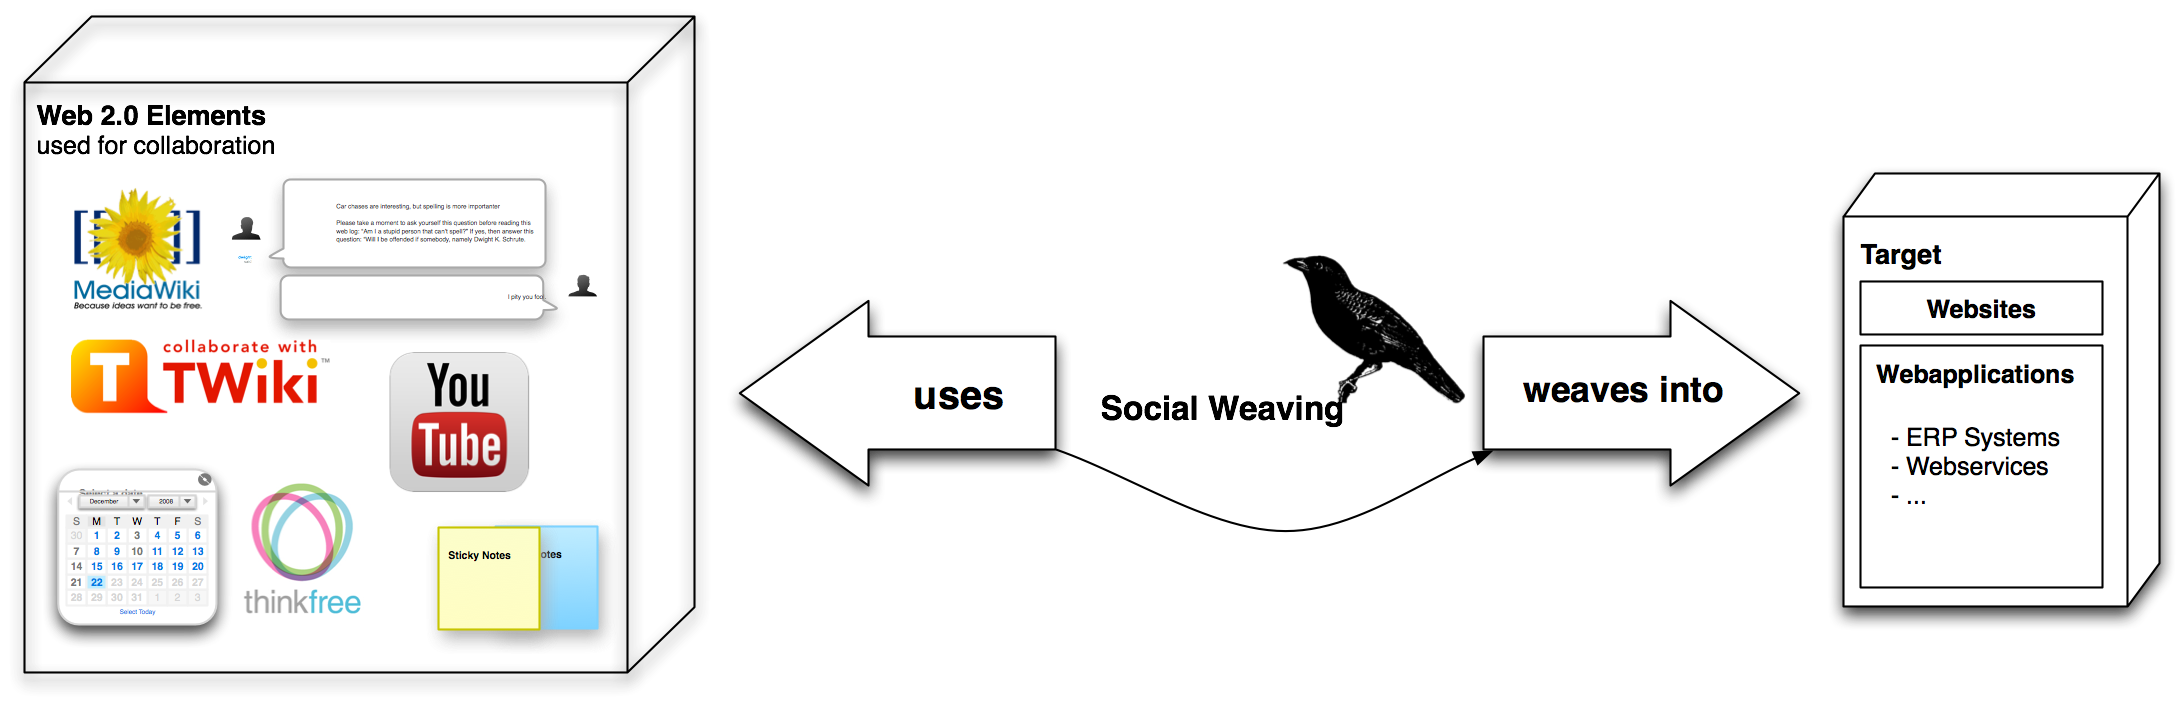
\includegraphics[width=13cm]{images/idead-social-weaving.png}
		\caption{Basic idea of Social Weaving}
		\label{idead-social-weaving}
\end{figure} 


So in combination we want the possibility to create some form of communication functionality - directly related to the button. And which is visible to a group of users for optionally unlimited amount of time.

Well if the web application would have an implemented comment box beneath the button, that would solve the problem. But that  solution brings another bunch of disadvantages. It would require to modify the web application that includes this functionality. And we cannot add comment boxes, links, ... to any element just as precautionary measure. This attempt of solution is not an option. 

What if we would have the opportunity to inject social elements directly into our web application without the need to modify it. Basically web applications run in a browser and what is displayed can be modified locally. And that is what we do. We weave social elements into the browser view and synchronize it for different user sessions. This way we reach exactly the functionality we need to solve our problem without touching the web application. We call this process Social Weaving. 

Even though Social Weaving overcomes the above mentioned problems - it confronts us with new types of pretty unpleaseant difficulties. Different browser types, unreliable web development styles, complex web technologies, etc. are examples for hurdles that Social Weaving has to deal with. 

This thesis will show what is possible with Social Weaving and where its boundaries are. 

In the following we are first going to discuss the idea of Social Weaving based on  an abstract requirements analysis of a prototype. What functionality does it need to achieve the goals we mentioned above and what are the difficulties? In the second part we are going down on a concrete level where we take the theory from the first part into action and actually explain the architecture and implementation of the prototype, Social Weaver, in detail. 
\newpage

\section{Requirements Analysis}\label{req-analysis}

\subsection{What is Social Weaver}\label{what_is_sowe}
Social Weaver (SoWe) is the name of a prototype system that weaves social web features into web applications. The system consists of a firefox plugin and the server side.

\begin{figure}[h!] \centering
		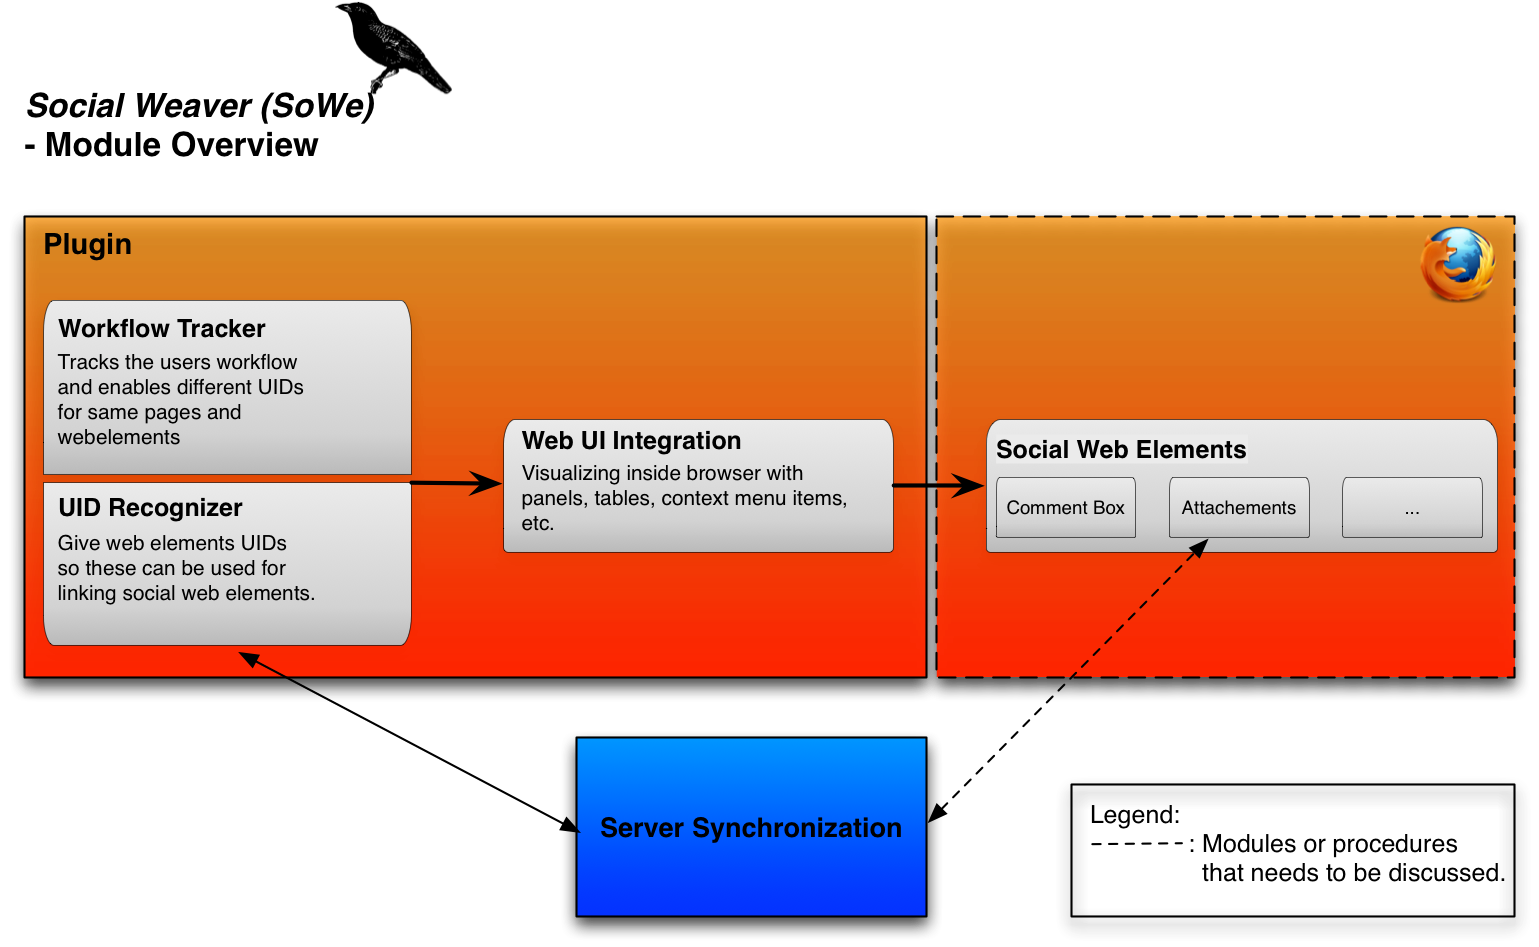
\includegraphics[width=13cm]{images/sowe-module-overview.png}
		\caption{Social Weaver Module Overview}
		\label{msowe-module-overview}
\end{figure} 

The plugin takes control of one or multiple user sessions and draws the additional content into the browser view. The server application synchronizes with each plugin and distributes updates between several clients. 

For a better understanding lets step through a generic use case where a user just opens a web application and modifies some content. The use case enumeration is related to the figure \ref{sowe-prototype-use-case}.

\begin{enumerate}
\item The user opens a web application
\item The SoWe-Plugin sends a notification to the server with all necessary information like user identifier, timestamp, ...
\item After the server receives the plugin message it synchronizes it with its current content in the database
\item The server application responses to the plugin client with content data if some exists
\item The plugin uses the content information from the server to insert all social web elements
\item The user decides to make some changes to the social web content (e.g. adds a comment or creates a new comment box)
\item Again a notification is being sent to the server with containing the changes
\item Server synchronizes the updates and responses
\item Plugin redraws the synchronized content
\end{enumerate}

\begin{figure}[h!] \centering
		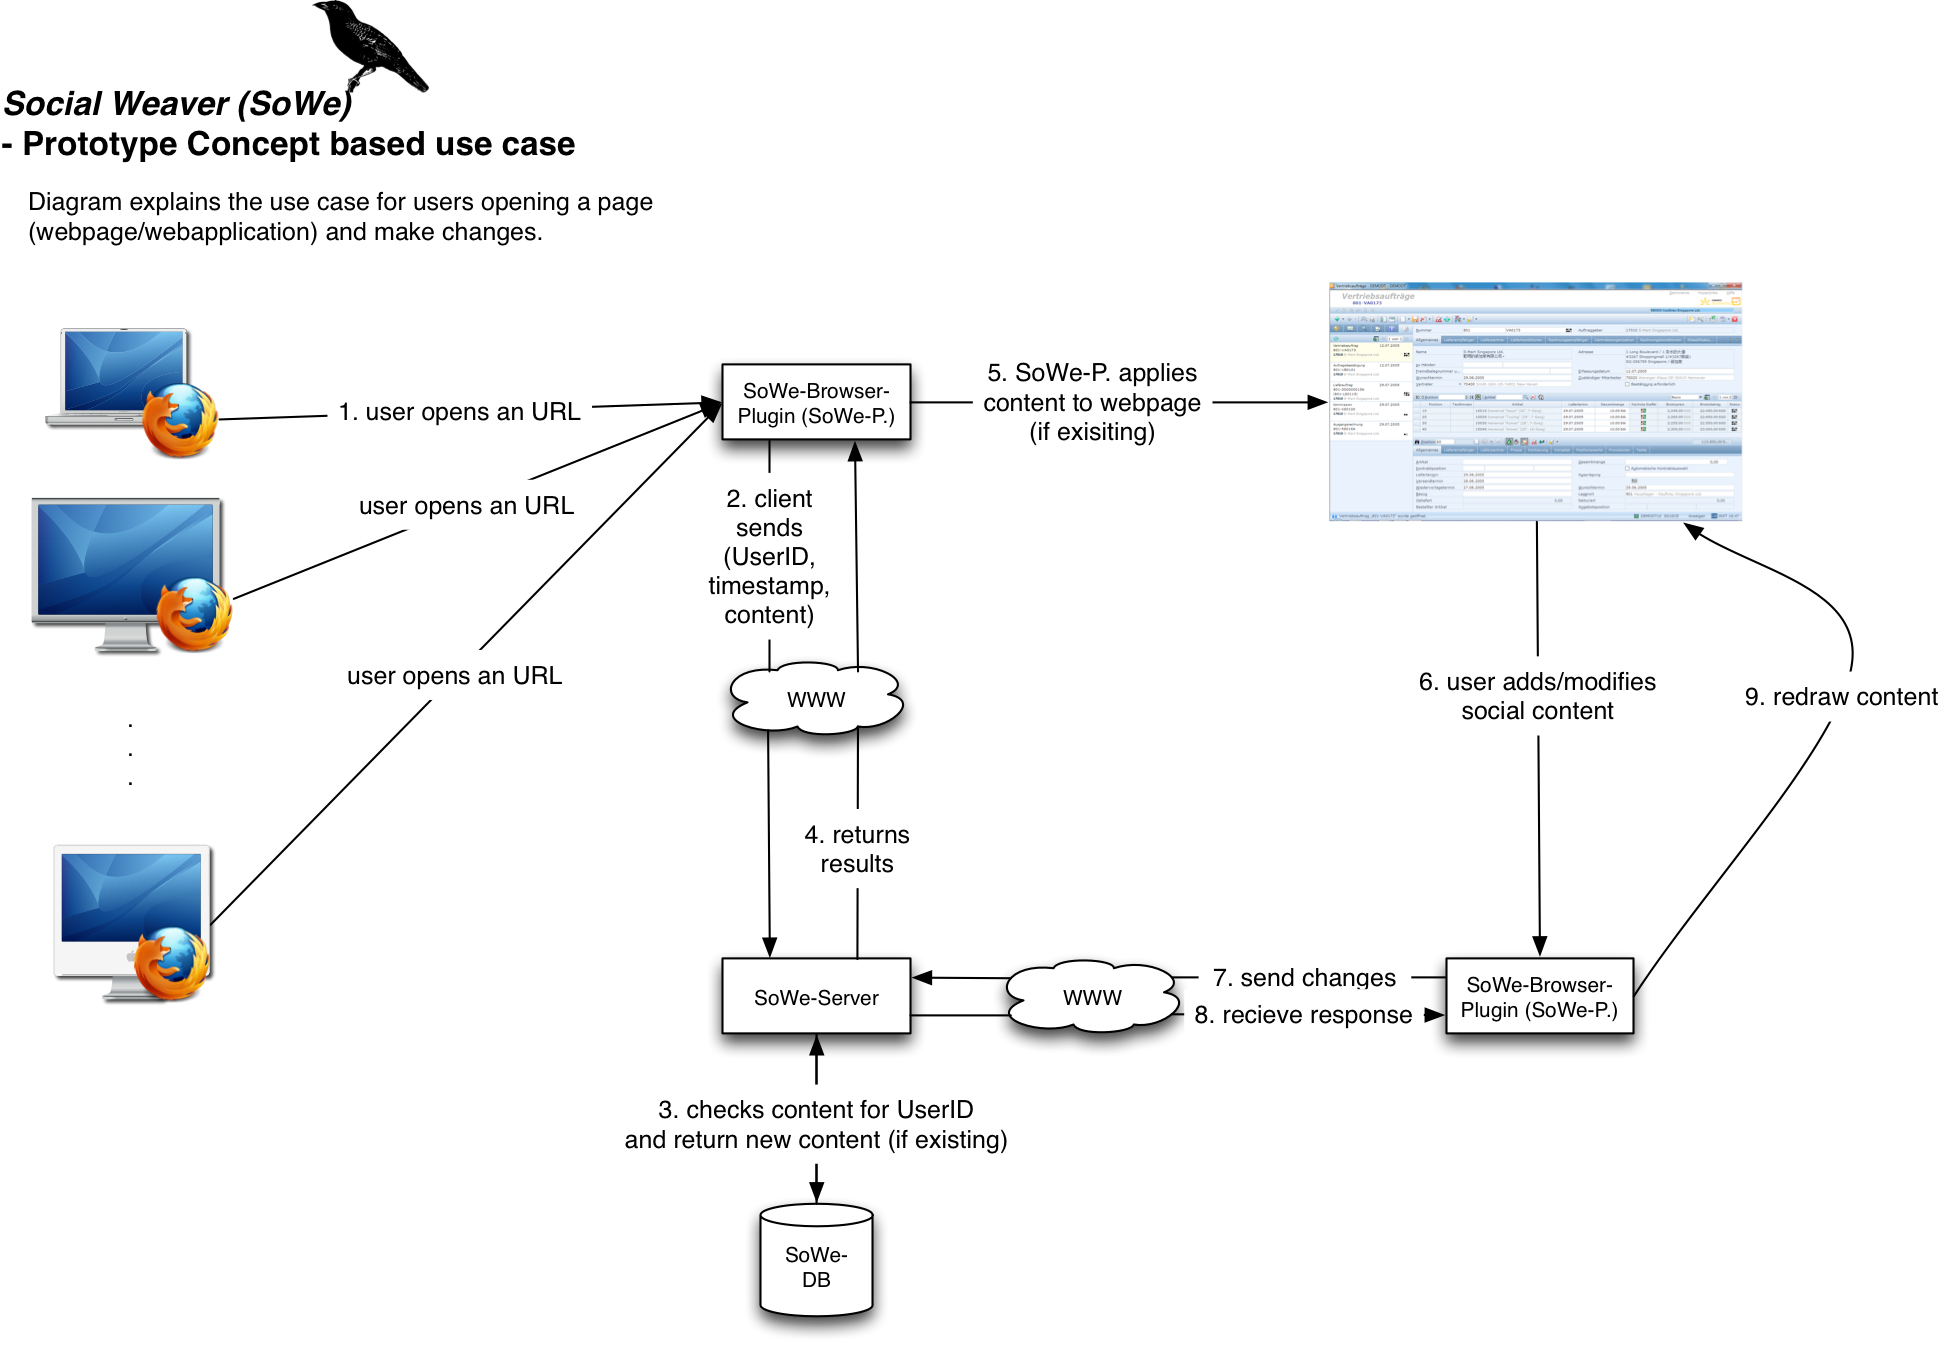
\includegraphics[width=13cm]{images/sowe-prototype-use-case.png}
		\caption{Social Weaver Prototype Use Case}
		\label{sowe-prototype-use-case}
\end{figure} 

\subsection{Requirements for Social Weaver}\label{sowe-reqs}

The general goal for Social Weaver is to weave social web 2.0 features into web-based applications. Since this is a broad requirement and impossible to be applied to any web application right from the beginning; it is necessary to break it down for the prototype.

More specifically the primary goal should be to get a system, that weaves one social web feature into a specific web application. SoWe has to be designed in a modular way, so that it will be possible to add more social media features, support multiple platforms and more web applications. Now that we have a rough idea what SoWe is going to be, lets list some concrete high-level requirements:

\begin{enumerate}
\item Browser plugin that supports a comment box
\item Server application that stores and synchronizes data that it receives from different client-plugins
\item Data format for storing and processing data for social web content
\item Communication protocol between plugin and server
\end{enumerate}

With these requirements we can start to specify our enlisting in detail:

\subsubsection{Browser Plugin}\label{browser_plugin}
In the following we define requirements on a abstract domain level according to \cite{van2009requirements}. A specification to a concrete domain level will follow in section \ref{firefox_plugin_requirements}, where we have specified what technologies to use.

As already mentioned the main requirement is that the plugin supports a comment box. That means that the browser has to display a comment box that is related to specific web element. For example in an online calendar an user adds a comment box related to an appointment that he wants to discuss in detail. 
Because it should be possible to add multiple comment boxes to any web element, we cannot just drop a box inside the user view, overlapping other interesting parts of the web application. Hence we have the requirement to make additional content visible to the user without interfering with the view on the original content. Possibilities would be fold/unfold-windows or just using small icons as references in the original view and outsource additional social content in external windows.

Of course the plugin needs to be able to communicate to the server application as well. (The server application is explained in the next section: \ref{Social Weaver - Server Application}). First of all the plugin needs to receive data that it print to the screen. Secondly changes made by the user has to be reported to the server. Because we are distributing the information between several users, there is also a need for synchronization. User updates may not overwrite updates made by other users etc.

The parser framework will contain application programming interfaces that create and parse the content of our tuples. This way it will be easier to add plugins for other browsers for instance. 
The data in the content-part of our tuple should have a uniform format no matter what web application or browser is in use. The server application will not need to know anything about the environment the plugin works in - it manages the social web content independently.

Another tricky and important point is the interaction with the web application. Most such sites are dynamic and there exists no static URLs we can refer to. And it is not certain that the same element, that two users refer to in their independent sessions, will have a comparable identifier. This issue definitely needs to be handled specifically for any web application. The good news is that this only affects the plugin. The server application just needs clearly defined identifiers. As a solution for the plugin we will need the possibility to use scripts for identifying elements. For example a script that supports the google calendar will be injected to make the plugin identify same appointments in different user sessions. This requirement is probably the vastly problematic one because it prevents a general usage of Social Weaver.

Lets summarize all the requirements we gained in this section:

\begin{enumerate}
\item Displaying and managing a comment box related to specific web element
\item Managing several comment boxes without disturbing the view on original content
\item Communication to server application
\item Creating Anchors
\item Creating content in uniform sending format
\item Parsing content from uniform sending format
\item Identifying web elements across different user sessions
\end{enumerate}

\subsubsection{Server Application} \label{Social Weaver - Server Application}
The server applications primary requirement is to synchronize different user sessions on one or multiple web applications. A user session is defined within the plugin (which does not mean a plugin can manage only one session). The server basically receives messages from different sessions, synchronizes them and distributes the most current state to all sessions.  To establish a lossless synchronization every message contains a timestamp.

We are assuming that every message contains an user identifier, a timestamp and an unique identifier for an element within the web application. This Anchor is the unique identifier for a single user action. For example if a user adds a comment to an already existing comment box that is related to an appointment in a calendar, the server receives the users identifier, the timestamp for the modification and an identifier for the appointment in the calendar. With this information the server can check its database for the comment box and add the new comment. 

It is important to remember that the server only uses the received data as identifier. All actions are completely independent to the web application. 

Also we may assume that the received message have the same Anchor form as discussed in the previous section. 
\begin{verbatim}(user identifier, timestamp, content)\end{verbatim} 
The content part from the Anchor will already be in a uniform that has been generated by the plugin. So even the browser type will not matter to the server. The server has to be able to parse the content package and to create a new one that can be parsed by our plugins.

So the requirements for the server application are:
\begin{enumerate}
\item Offer service that receives messages from plugin-clients
\item Synchronization for requests from different user-session
\item Persist updates into a database
\item Keep the server application independent to weaved-into web application
\item Parse incoming messages
\item Create outgoing messages
\end{enumerate}


\subsubsection{Communication Protocol}\label{communication_protocol}


\subsection{Technologies}
This section should provide a short overview about the technologies that are being used for Social Weaver. 
\begin{itemize}
\item Firefox plugin API
\item REST as Web service Interface
\item JavaEE for server application 
\item PostgreSQL for persistence layer
\item JSON for formatting data
\end{itemize}

\newpage

\section{Social Weaver - Implementation Level}\label{sowe-concrete}
So far, however, the previous section operates on a Meta level. Abstract requirements describe universally a Social Weaving system without going into detail or explaining the prototype. The coming section use the results, gathered on the conceptual level, for the development of the prototype, Social Weaver. 
Each module is illustrated separately. Ahead the technologies are explained that are used in the given modules. Finally, for each module the brief architecture and some interesting aspects are mentioned. 

\subsection{Social Weaver - Firefox Plugin} \label{sowe-firefox}
This section briefly explains what technologies we use for Firefox plugin development and describe in detail how the Social Weaver plugin is implemented.

\subsection*{Firefox}
Firefox is a free web browser that has been released 2004 by the Mozilla Foundation\footnote{\url{www.mozilla.org}}. It is being distributed under multiple licenses under Mozilla Public License (MPL)\footnote{\url{http://www.mozilla.org/MPL/1.1/}}, GNU Lesser General Public License and GNU (LGPL)\footnote{\url{http://www.gnu.org/licenses/lgpl-3.0.de.html}} General Public License (GPL) \footnote{\url{http://www.gnu.org/licenses/gpl-3.0.html}}. 

The reasons why we chose Firefox as prototype environment are the high distribution of the browser and an easy extend ability with plugins, and extensions.

\subsection*{Firefox Plugin Development}
To improve readability of the coming Section \ref{firefox_plugin_requirements} \nameref{firefox_plugin_requirements}, we discuss some aspects from the Mozilla Add-on SDK (Version 1.13) \footnote{\url{https://addons.mozilla.org/en-US/developers/docs/sdk/latest}}. Readers who are not interested too much into technical detail or are familiar with the technologies can skip this section.

The used methods aren't just explained independently but brought into context to our prototype planning so it becomes clear what purpose they have. 

The Add-on SDK allows creating add-ons for the browser using the most common web technologies (like HTML, CSS, JavaScript, etc.). Furthermore, it provides a low level API and a high level API set. The most important interfaces that are being used for our prototype are High-Level-Interfaces and are explained in the following.

\begin{description}
\item Panel\\
A \emph{panel}\footnote{\url{https://addons.mozilla.org/en-US/developers/docs/sdk/latest/modules/sdk/panel.html}} is very flexible dialog window. Its appearance and behavior is specified by a combination of a HTML and a JavaScript file. Additionally a CSS file might be used to change the look even further. The limitations of a panel are the limitations of the mentioned technologies. 
A panel is meant to be visible only temporarily and easy to dismiss because any user interaction outside the panel.

\begin{figure}\centering
		
\includegraphics[width=7cm]{images/example-panel.png}
		\caption{An example for a \emph{panel} that shows a list of annotations}
		\label{example-panel}
\end{figure} 

We use the \emph{panel} for getting user input, displaying information (like in screen shot \ref{example-panel}) and to integrate our social media web elements. 

Actually the flexibility of \emph{panel} is the reason why our prototype is able to support social weaving for basically any web element that can be represent in HTML code. Still it is necessary to embed the external HTML code, which may leads to boundaries and difficulties.

\item Simple-Storage\\
This module\footnote{\url{https://addons.mozilla.org/en-US/developers/docs/sdk/latest/modules/sdk/simple-storage.html}} is an easy to use method to store basic properties (Booleans, numbers, strings, arrays, ...) across browser restarts. 

With an operation like

\begin{lstlisting}
var ss = require("sdk/simple-storage");
ss.storage.myNumber = 41.99;
\end{lstlisting}

we store a number like an object and can it access just as easy like that. The price for such a simple usage is paid with high limitations. For instance, searching is not possible. Nevertheless, we can store an array and search the array. 

That is exactly how we store our annotations for our prototype. More details are provided in the next section.

\item Page-Mod\\
The \emph{page-mod}\footnote{\url{https://addons.mozilla.org/en-US/developers/docs/sdk/latest/modules/sdk/page-mod.html}} module enables us to act in a specific context related to a web page. Then it becomes possible to attach Java Scripts to it and to parse or modify certain web page parts.

In our context we are going to use \emph{page-mod} to parse the HTML code to find elements that can server as anchors for annotations. Moreover, of course to find elements those are already annotated.

\item Widget\\
The module that is called \emph{widget} \footnote{\url{https://addons.mozilla.org/en-US/developers/docs/sdk/latest/modules/sdk/widget.html}} is simply an interface to the Firefox add-on bar\footnote{\url{https://developer.mozilla.org/en-US/docs/The_add-on_bar}}. It is possible to attach \emph{panels} and trigger operations by clicking the \emph{widget}. 

\begin{figure}\centering
		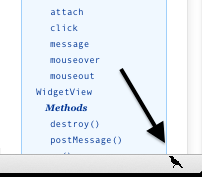
\includegraphics[width=7cm]{images/example-widget.png}
		\caption{Example for a widget serving as activation button}
		\label{example-widget}
\end{figure} 

We use a widget to switch between different modes (see coming Section \ref{display-management-requirement} for more details about how the mode-system works).

\item Self\\
\emph{Self}\footnote{\url{https://addons.mozilla.org/en-US/developers/docs/sdk/latest/modules/sdk/self.html}} provides access to add-on specific information like the Program ID\footnote{\url{https://addons.mozilla.org/en-US/developers/docs/sdk/latest/dev-guide/guides/program-id.html}}, which is important for an official distribution of the add-on. More meta information like the name or the version are accessible via the \emph{self} module. Also bundled external files are integrated by \emph{self}.

Even though it is an important module for the plugin - there is no specific relation to the used system. 

\item Notifications\\
This module\footnote{\url{https://addons.mozilla.org/en-US/developers/docs/sdk/latest/modules/sdk/notifications.html}} displays toaster\footnote{Toasters are commonly called notifications that just appear, or slides in the users view - like a toast hops up.}-messages\footnote{\url{http://en.wikipedia.org/wiki/Toast_(computing)}} that disappear after a short time.

We use these to keep the user informed without bothering him too much by forcing him to dismiss trivial notifications.

\item Request\\
This simple to use, but yet powerful module \emph{request}\footnote{\url{https://addons.mozilla.org/en-US/developers/docs/sdk/latest/modules/sdk/request.html}}, enables us o perform network requests. Once we create a \emph{Request} object we can specify whether it is a GET, PUT or POST request. These request types are specified by the REST standard so any web service that supports REST is able to interact with this module\cite{fielding2000principled}. The response from a server is directly accessible like any other JavaScript object. 

We are going to use \emph{request} for our communication with our synchronization web service. This includes sending updates, made with the plugin instance, to the server and receiving updates that were made in other sessions or with different plugin instances, from the server. 

\end{description}

\subsubsection*{JQuery}
\emph{jQuery}\footnote{\url{http://jquery.com/}} is a free JavaScript library under the MIT License\footnote{\url{http://www.mit.edu/}} that offers many functions for modifying DOM trees. It has been released 2006 in context of a BarCamp\footnote{\url{http://en.wikipedia.org/wiki/BarCamp}} in New York.

Even though this library is not a part of the Mozilla Add-on SDK it is being heavily used by it. Any operation that changes or traverses the HTML code (like changing the background color of web elements) is being reached with jQuery.

The reason why jQuery makes it so easy to handle operations on HTML code is based on the selector that searches the DOM tree. Most jQuery operations are based on elements in the DOM tree. With the selector \verb+jQuery()+ (which can be equally written as \verb+$()+) any element in the DOM tree can be used to create a jQuery object. This object can be used to perform modifying operations on it. For instance, we step through the following short operation:
\begin{lstlisting}[language=JavaScript, numbers=left]
$('.user-name').click(function(){
   this.empty();
});
\end{lstlisting}

In line one we use the \verb+$+ selector to find any element in the DOM tree that has the id \verb+user-name+. Since we use the jQuery selector, any found element can be handled as a jQuery object. This way \verb+click(function(){...})+ appends a click observer to all elements. Any time one of those elements is clicked by the user, this triggers the function. This function includes \verb+this.empty()+, which only removes all content inside the element. 

Another and more related example of jQuery usage is used in the selection part of the plugin:
\begin{lstlisting}[language=JavaScript, numbers=left]
$(":visible").filter(function(index) {
  if(this.content()){
      return true;
  }else{
      return false;
  }
}).mouseenter(function() {...}
\end{lstlisting} 

First of all we request all elements that are visible to the user by using \verb+$(":visible")+. Because it is unlikely that a user tries to select an element without any content - we filter all elements from the result set that are empty. (Such elements can be placeholders, flexible empty space and so on.) Now that our results contains mostly relevant elements to the user, we append \verb+.mouseenter()+ to recognize when the courser is placed above the element. The skipped function itself contains operations to recognize more user operations and element analysis. To discuss more code in detail would be beyond the frame. 

We only have seen a brief overview about jQuery operations. To fully understand how the prototype works and to operate with the script support it is advised to gather a better overview using, for instance, the official W3 introductions: \url{http://www.w3schools.com/jquery/}. 

\newpage
\subsection{Requirements for the Plugin}\label{firefox_plugin_requirements}
Let us recap what requirements we gathered in Section \ref{browser_plugin} on the conceptual level \cite{van2009requirements}:

\begin{enumerate}
\item \reqPi
\item \reqPii
\item \reqPiii
\item \reqPiv
\item \reqPv
\item \reqPvi
\item \reqPvii
\end{enumerate}

In the following concretion we apply the conceptual requirements to our environment which is the \emph{Mozilla Plugin Development SDK} \footnote{\url{https://addons.mozilla.org}}. In the following, we handle each requirement, mentioned above, separately:

\subsubsection[Visualizing]{\reqPi}\label{display-management-requirement}
Obviously "Displaying and managing a comment box related to specific web elements" consists of multiple sub requirement that we need to distinguish. 

\begin{figure}\centering
		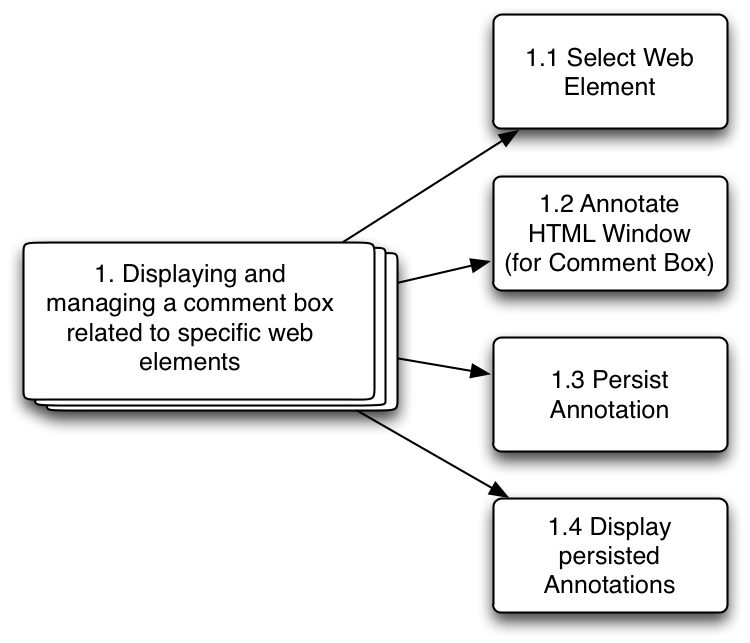
\includegraphics[width=10cm]{images/abstract2concrete-1.png}
		\caption{Partition of the first plugin requirement to sub requirements}
		\label{abstract2concrete-1}
\end{figure} 

Before we are able to annotate something, we first of all need a function to select or recognize a web element the users cursor points to (check 1.1 in Figure \ref{abstract2concrete-1}). \emph{Selecting} in this context means that we analyze the Document Object Model (DOM)\footnote{\url{http://www.w3.org/DOM/}} tree. The selection itself is easy to implement using the function \emph{mouseenter} and \emph{on('click')} from jQuery library\footnote{\url{http://jquery.com/}}. It becomes problematic to find this element again without any user interaction. Therefore, we need to set well chosen parameters that are used to determine the element. Next time we need to find the element - only the parameters can be used to find the element in the DOM tree. This issue is topic in the Section \ref{sowe-script-support} \nameref{sowe-script-support}.

Theoretically, it could be possible for user to select any element in the web view - but practically this would make the selection procedure confusing for development as well as for the user. Therefore, we apply some filters. Elements like empty boxes and placeholders are not selectable. 
Still it should be clear to the user what he might select. 

To achieve this functionality we create thin rectangles around every element that is a selection option. These rectangles only appear for time the plugin is in selection-mode and disturb the web view just for a certain time. More on the different mode types in \ref{user-disturbance} \nameref{user-disturbance} .

Now that we can locate a specific web element, we may annotate some social web element. For reasons of flexibility and simplicity we just annotate a HTML window (check 1.2 in Figure \ref{abstract2concrete-1}), where we can inject any external HTML code. The Mozilla SDK high-level APIs \footnote{\url{https://addons.mozilla.org/en-US/developers/docs/sdk/latest/modules/high-level-modules.html}} offers all necessary tools to insert a HTML box as a \emph{Panel}\footnote{\url{https://addons.mozilla.org/en-US/developers/docs/sdk/latest/modules/sdk/panel.html}}.

The annotation anchors are visible to the user in form of a colored background that we create by modifying the DOM tree.
If the user clicks on such an element the already existing panel is opened. 

\begin{figure} \centering
		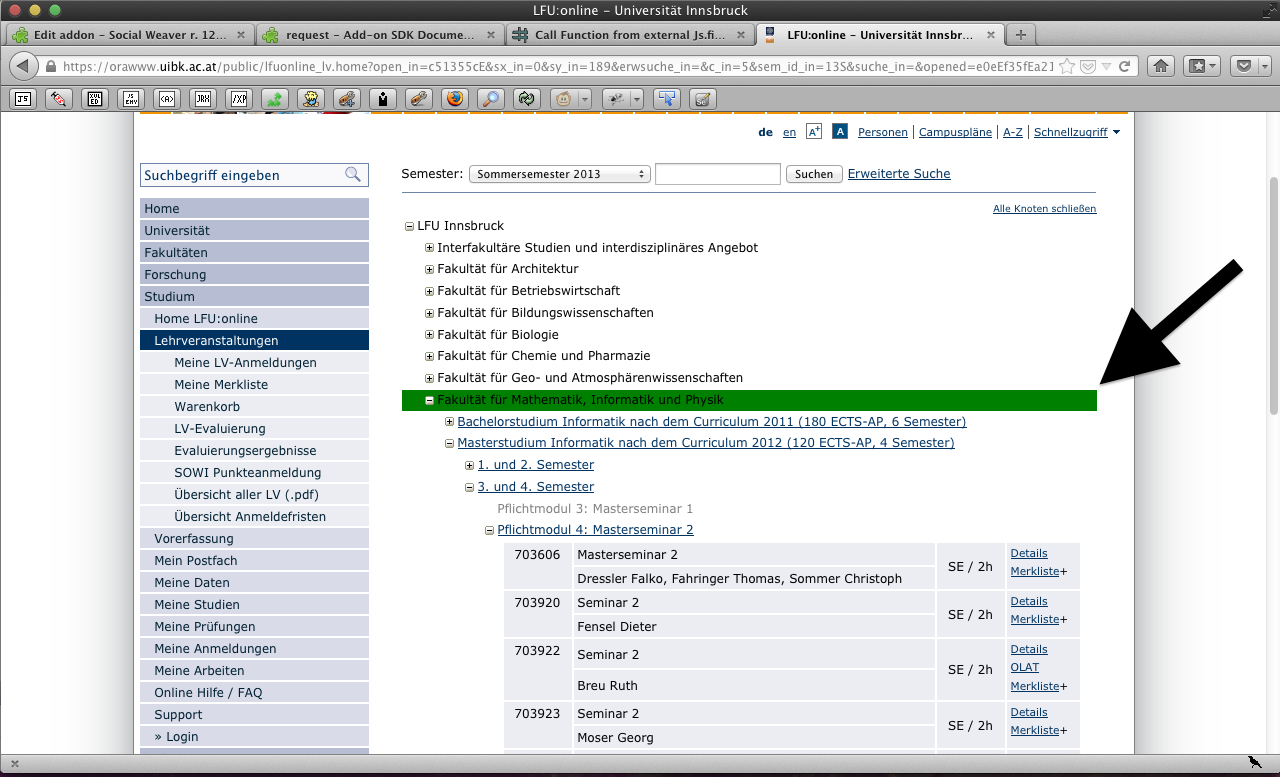
\includegraphics[width=13cm]{images/annotation-rectangle-sample.png}
		\caption{Rectangle shows that the underlying element is possible for annotation}
		\label{annotation-rectangle-sample}
\end{figure} 

To decouple our annotated data (like anchors, annotations, ...) from the actual synchronization, which is covered later, we want to use a storing system that is also provided by the Mozilla SDK (see 1.3 in Figure \ref{abstract2concrete-1}). The high level API \emph{simple-storage} \footnote{\url{https://addons.mozilla.org/en-US/developers/docs/sdk/latest/modules/sdk/simple-storage.html}} enables us to store all information we need and recall them. Just the synchronization mechanism should modify this data set. All displaying procedures should be outside of server communication reach. This means that if an annotation is created, the changes are written locally into the plugin local data storage. Only after the persistence is complete, the synchronization procedure is initiated. While synchronizing, the changes are transmitted to the server. 

The last sub requirement is to re display existing annotations (check 1.4 in Figure \ref{abstract2concrete-1}) from our \emph{simple-storage}. Besides using the same techniques for drawing content and retrieving it from the storage, we need to match the web page content to our saved annotations. For that we use a matcher instance that checks the DOM tree for IDs that we are already using. 

This is actually only trivial on a very simple basis. Let us assume that we have more than one element attached to the same web element. Or we have different user sessions and/or include a workflow so that we need to distinguish the same element for different instances of the web page. In that case generating reliable IDs becomes quite complicated. Nevertheless, these issues just affect the way we assign IDs to elements and how we retrieve them. The requirement 1.4 is just about matching existing IDs to a web page. 

As already mentioned we use a matcher that checks the DOM tree for IDs. In case we have an anchor in our \emph{simple storage} then we modify the web page HTML code similar as we did for requirement 1.1. Visual differences are that we do not modify the background of an element but generate an rectangle around it instead (see screen shot in Figure \ref{annotation-rectangle-sample2}). 

\begin{figure} \centering
		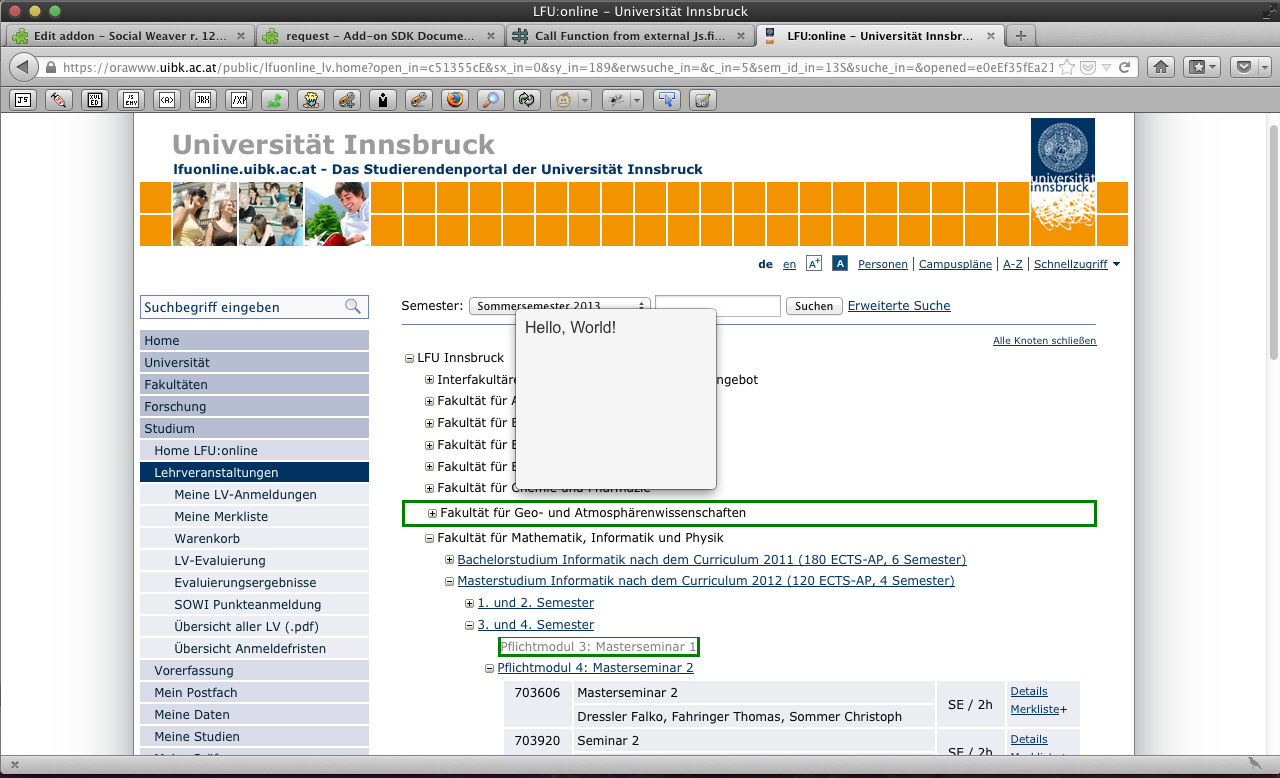
\includegraphics[width=12cm]{images/annotation-rectangle-sample2.png}
		\caption{Rectangle shows that the underlying element is possible for annotation}
		\label{annotation-rectangle-sample2}
\end{figure} 

This way we are able to show the user which elements are annotated. Of course, without further information, it is not obvious what is annotated exactly. What we need is anno easy to access functionality so that the user can find out what the annotation is. 

For that reason we modify the above mentioned matcher class to generate a panel in case the user performs a \emph{mouseenter} operation. This panel should show a brief version of the attached social element. In our case it could be the name of the context the comment box is related or the names of the attendees (our example screen shot just print outs "Hello, World!" \ref{annotation-rectangle-sample2}). 

\subsubsection[User View Management]{\reqPii}\label{user-disturbance}

This requirement ensures a positive user experience, but is not directly about functionality. It is possible to attach annotations to nearly any element in a web application. This is a lot of potential additional footage. Nevertheless, the user needs to be in the position to navigate like usually within the application. 

There are two options to guarantee such a requisition. Either we minimize the overhead that we display into the web view or we display additional information only at the appropriate time. To achieve the best results we combine both possibilities by introducing the mode system:

The plugin has several modes that support different functionality and show different content. Those modes can be switched by clicking the widget in the add-on bar. Every mode has its own logo, see Figure \ref{mode-logos}. 

\begin{figure}\centering
		
\includegraphics[width=13cm]{images/mode-logos.png}
		\caption{Widget representation for different modes}
		\label{mode-logos}
\end{figure} 

We distinguish the following modes:
\begin{enumerate}
\item Default mode \\

In the default mode, the plugin runs passively. It does not disturbs the user but runs synchronization and matching procedures in background. When the user opens a new web view, the plugin checks its database for annotations that belong to the view. If a positive match is found, it is into the users web view. 

The navigation of the browser is as usual, except for the annotations that include a click handler that triggers the function for opening the social element.

\item Selection mode \\ 

The selection mode interferes eminently with the navigation and the representation of the regular browser view. Activating the selection mode marks all selectable elements with rectangles around it. Moving the cursor around the web view additionally marks the element beneath the cursor to visualize what element is marked when clicked. 
In this  mode clicking links and buttons and, does not trigger the functionality of those elements but instead select them so an annotation might be created. 

Disabling the selection mode clears the view from the previously mentioned marks. Only successfully created annotations remain persistent. 

\item Deactivated mode \\ 

Deactivating the plugin entirely disabled any functionality. This can be useful in worst cases like that the plugin prohibits regular navigation or the annotation marks interfere with the users view.
\end{enumerate}

The mode system could be a starting point for extending Social Weaver for multiple user sessions in one plugin context. Alternatively, providing securely authenticated sessions that can only be activated when correct credentials is provided. 

\begin{figure}\centering
		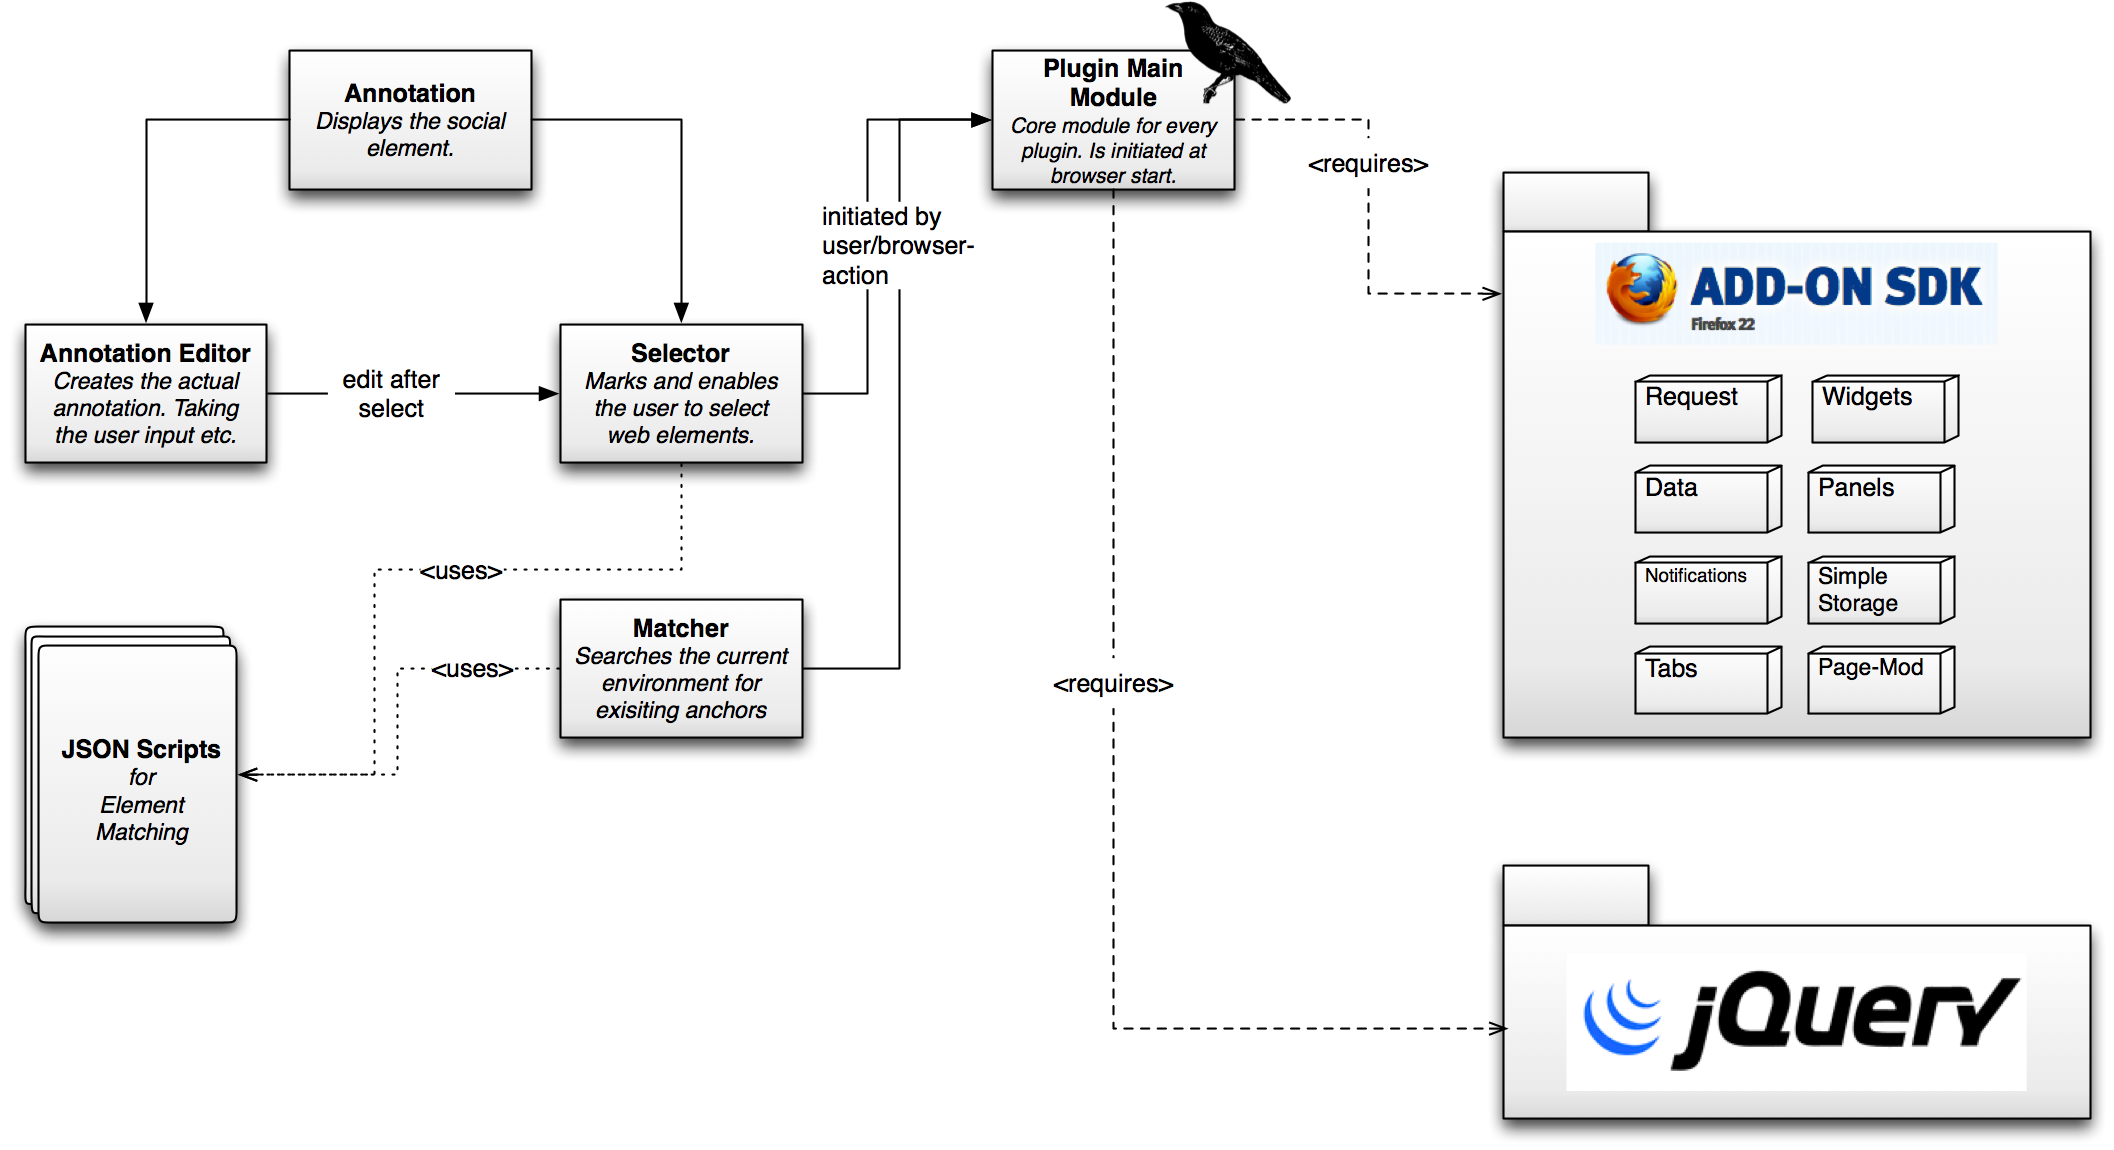
\includegraphics[width=13cm]{images/plugin-architecture.png}
		\caption{Architecture of the Firefox Social Weaver Plugin}
		\label{plugin-architecture}
\end{figure} 

\subsubsection[Communication]{\reqPiii}
To share our comments or annotations with other users we need a server side synchronization procedure. This section is only about the requirements that are related to the plugin side. (Details to the web service are discussed in \nameref{ws-architecture-intro} \ref{ws-architecture-intro}.)

The first step to achieve this goal is to establish a communication between the plugin and a web service. For this purpose we are going to make use of the \emph{request} module from the Mozilla Add-on SDK. It provides an easy to use JSON\footnote{\url{http://www.json.org/}} and REST(\cite{fielding2000principled}) assistance. 

We split this into the following sub requirements:
\begin{description}
\item Plugin receives updates from server\\
What the plugin needs to know from the server is a set of Anchors. Those Anchors contain information like the author identification, a time stamp and of course the content.
(see \ref{creating_triplets}) 
So at this point we assume that our server provides a set formatted in JSON. The plugin generates a request to retrieve this data. 
\begin{figure}
\begin{lstlisting}[language=JavaScript]
var sync = Request({
      url: 'http://localhost:9998/anchor',
      onComplete: function(response) {
        for(var i = 0; i<response.json.length; i++){
            var r = response.json[i];

            newAnchor = new Array(r.anchorURL, 
		r.ancestorId, r.anchorText);
            var newAnnotationText = r.annotationText;
            handleNewAnnotation(newAnnotationText, 
		newAnchor);
     };
   }
});
sync.get();
\end{lstlisting}
\label{anchor_sample_code}
\caption{Sample JavaScript code for retrieving JSON objects from a web service with a GET REST request}
\end{figure}

This goal is surprisingly simple to achieve. In the sample code \ref{anchor_sample_code} we just need to specify the URL of the web service and we are able to access the JSON objects right away exactly like JavaScript objects. Then we use the JSON objects to create an anchor entity and use the existing \verb| handleNewAnnotion(newAnnotationText, newAnchor)| method to store it in our \emph{simple-storage} list. 

Our prototype is a proof-by-concept system, therefore we keep the synchronization really simple. Instead of checking for new annotations and match them with the already existing data, we just rewrite our local plugin data set with a copy from the server. This technique could easily lead to corrupt and inconsistent data sets. However, since the prototype is not to be used for confidential data or in any real world scenario at all - we just take the risk.

\item Plugin sends updates to server\\
When a user creates a new annotation or modifies it - the plugin should send an update to the web service immediately. Again we set up a method using the \emph{request} module. 
\end{description}

\begin{figure}
	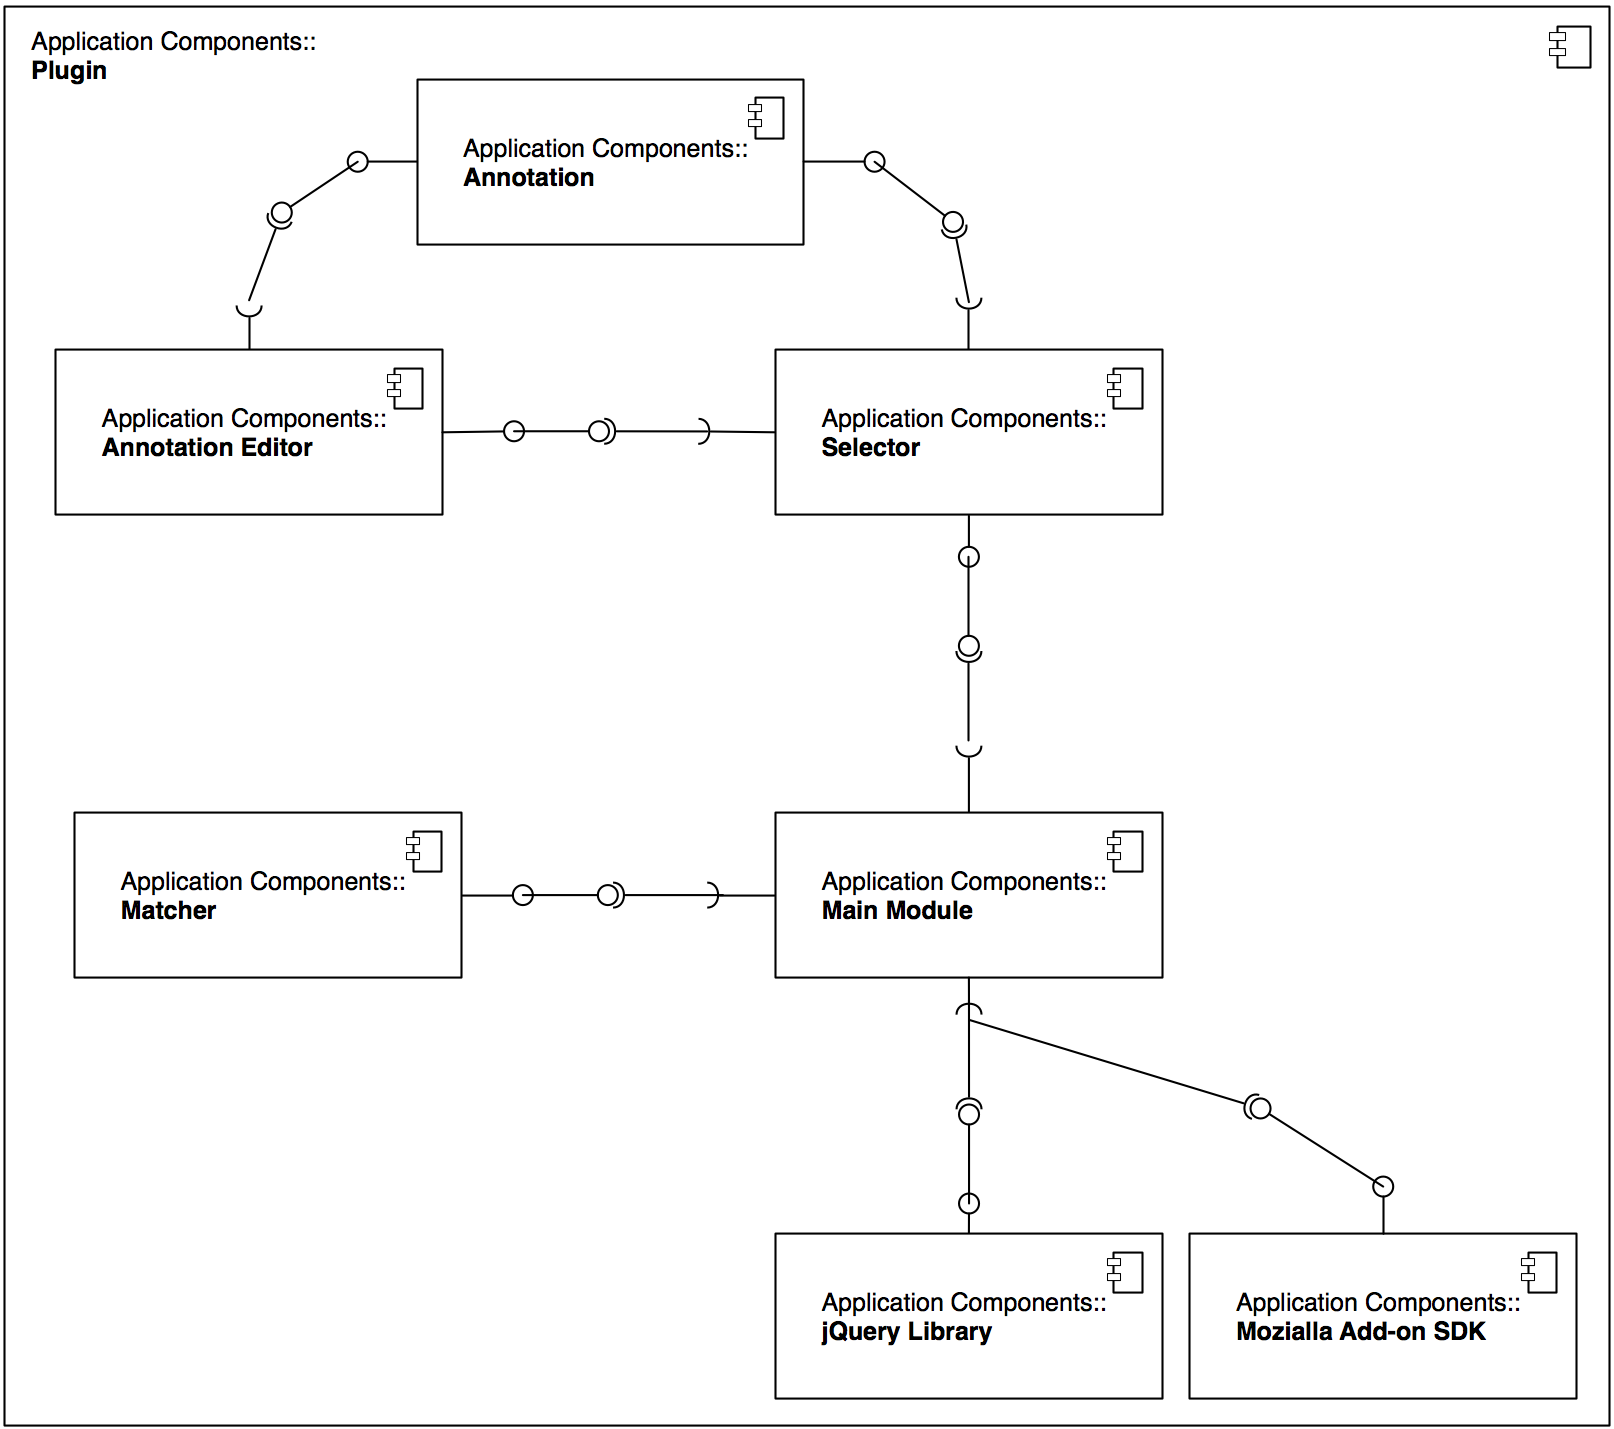
\includegraphics[width=11cm]{images/component-plugin-diagram.png}
	\caption{Component diagram for the plugin}
	\label{component-plugin-diagram}
\end{figure}

\subsubsection[Creating Anchors]{\reqPiv}\label{reqPiv}
We already mentioned anchors in the context of transmission. This section covers how those anchors are created at the plugin before sent to the web service. 
The first step in the creation of an anchor happens in the \emph{selector} after the user clicked an element. After this happens, every rule from the current script loads and executes, using the clicked element as input. The results are stored in an array we call payload. Once this process is finished we pass the payload with the current URL back to the \emph{main module}:

\begin{lstlisting}
event.preventDefault();    
        self.port.emit('show',[
            url,
            JSON.stringify(arr.payload)
          ]);
\end{lstlisting}
How the results contained by the payload look like, is discussed in the next Section \ref{reqPv}. 
The \textit{selector} is initiated in the \textit{main module}, providing a worker that is listening for the emission called \textit{show}. 
\begin{lstlisting}
worker.port.on('show', function(data) {
          annotationEditor.annotationAnchor = data;
          annotationEditor.show();
        });
\end{lstlisting}
From here we pass the anchor information to the \textit{annotation editor}. The editor is responsible for storing the user input that defines the social element. At this point, we just assume that, no matter what social element is annotated, it generates a string like value that we can use for processing. So the \textit{editor} extends the anchor data with the social element content. 

Now that the annotation and its anchor is complete we call:
\begin{lstlisting}
function handleNewAnnotation(anchor) {
  var newAnnotation = new Annotation(anchor);  
  simpleStorage.storage.annotations.push(newAnnotation);
  synchronize();
}
\end{lstlisting}

Temporarily we persist the new annotation in \textit{local storage}, and then start the synchronizing with the web service. The annotation is dismissed in case the synchronization fails. 


\subsubsection[Uniform Sending Format]{\reqPv}\label{reqPv}
The previous Section \ref{reqPiv} showed how an annotation and its anchor is generated. Now the content of those entities is topic. 

\begin{figure}\centering
	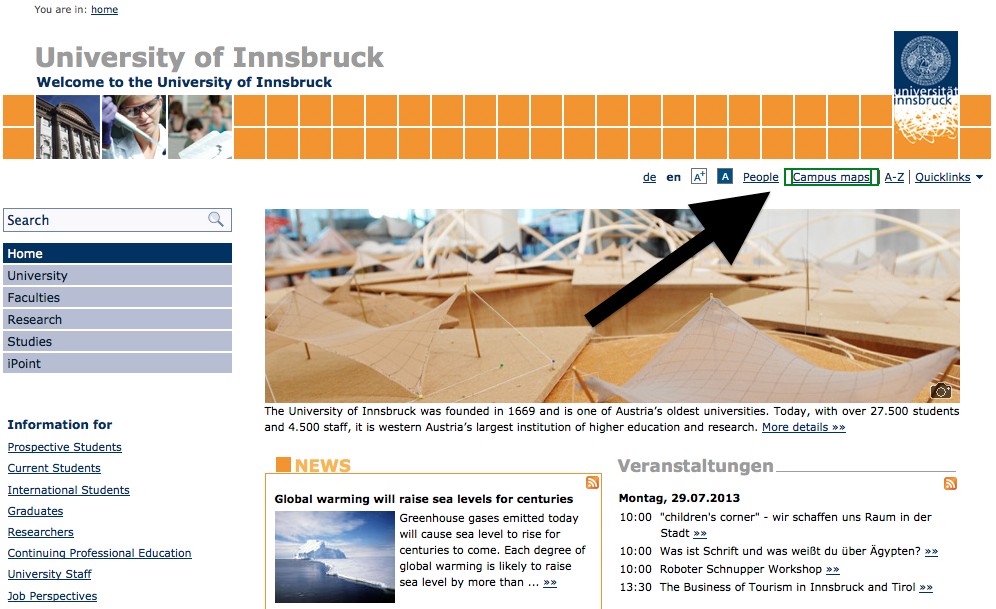
\includegraphics[width=10cm]{images/anchor-example-uibk.png}
\caption{User selects the element pointed by the arrow}
\label{anchor-example-uibk}
\end{figure}


Again the first step in creating an anchor is to gather results on the clicked element according to the script. To illustrate that, we show this on an example in Figure \ref{anchor-example-uibk}. 
Next we use the following script:
\begin{lstlisting}
{"rules": [
        {"doc_location": "document.location.toString()"},
        {"element_content": "matchedElement.text()"}
]}
\end{lstlisting}

Executing this script on the web element results in the payload below:
\begin{lstlisting}
 [
 	{"doc_location":"http://www.uibk.ac.at/"},
 	{"element_content":"Campus maps"}
 ]
\end{lstlisting}

Moreover we add the current URL to the annotation, which is redundant in that case with the rule \textit{doc\_location}, but not necessarily have to be in different cases. Thereafter we pass the coming information array to the \textit{editor}:
\begin{lstlisting}
{"annotation":[
	 {"url": "http://www.uibk.ac.at/"},
	 {"payload":[
 			{"doc_location":"http://www.uibk.ac.at/"},
 			{"element_content":"Campus maps"}
 	]}
 ]}
\end{lstlisting}

The \textit{editor} processes the user input and transforms it to a string that is added to the annotation. To keep the previous example tangible, we assume that the user creates a link to some wiki upon the element like: \url{http://www.uibk.ac.at/internalwiki/faqs}. 
Consequently the updated annotation contains something like:
\begin{lstlisting}
{"annotation":[
	 {"url": "http://www.uibk.ac.at/"},
	 {"payload":[
 			{"doc_location":"http://www.uibk.ac.at/"},
 			{"element_content":"Campus maps"}
 	]},
 	{"social_element":"http://www.uibk.ac.at/internalwiki/faqs"}
 ]}
\end{lstlisting}

This JSON array has the form, ready for being transmitted to the web service. The server side uses the data to create anchor and social element entities, but does not modify the values itself, unless it is an update. 

\subsubsection[Parsing Incoming Messages]{\reqPvi}\label{reqPvi}
Basically, parsing incoming messages is quite the analogous opposite to the creation and sending procedure in \ref{reqPv}. After the web service responds to the plugin request for updates, the incoming message is a JSON array of annotations. Formerly we have seen an example for such an annotation like:
\begin{lstlisting}
{"annotation":[
	 {"url": "http://www.uibk.ac.at/"},
	 {"payload":[
 			{"doc_location":"http://www.uibk.ac.at/"},
 			{"element_content":"Campus maps"}
 	]},
 	{"social_element":"http://www.uibk.ac.at/internalwiki/faqs"}
 ]}
\end{lstlisting}
Once the annotation list is received by the array, it is split and the single annotations parsed into its pieces: \textit{url}, \textit{payload}, \textit{social\_element}. Those are formed to an \textit{Annotation} object and persisted in local storage. 
\begin{lstlisting}
function updateAnnotation(anchor) {
  var newAnnotation = new Annotation(anchor);  
  simpleStorage.storage.annotations.push(newAnnotation);
  updateMatchers();
}
\end{lstlisting}
At last, the matchers need to be updated, so the new annotations are checked on coming web view. 

\subsubsection[Web Element Identification]{\reqPvii}
Some of the previously discussed requirements were prerequisites, so finally the most challenging requirement can become subject. 
For matching web elements, we need an annotation that has been created by a user selection. This process has been described in Section \ref{reqPiv}. This annotation has to be synchronized with the web service so other users are able to see the annotation as well. Formerly this was topic in Section \ref{reqPv}. 

In the first place, the element identification is done by the matcher. Every time a new web view is opened, the actual URL is passed to a matcher worker. A matcher worker is a thread-based instance of the matcher module. Using workers enables the plugin to run multiple matching procedures parallel (which is useful, for instance, when using tabs). 

\begin{figure}\centering
	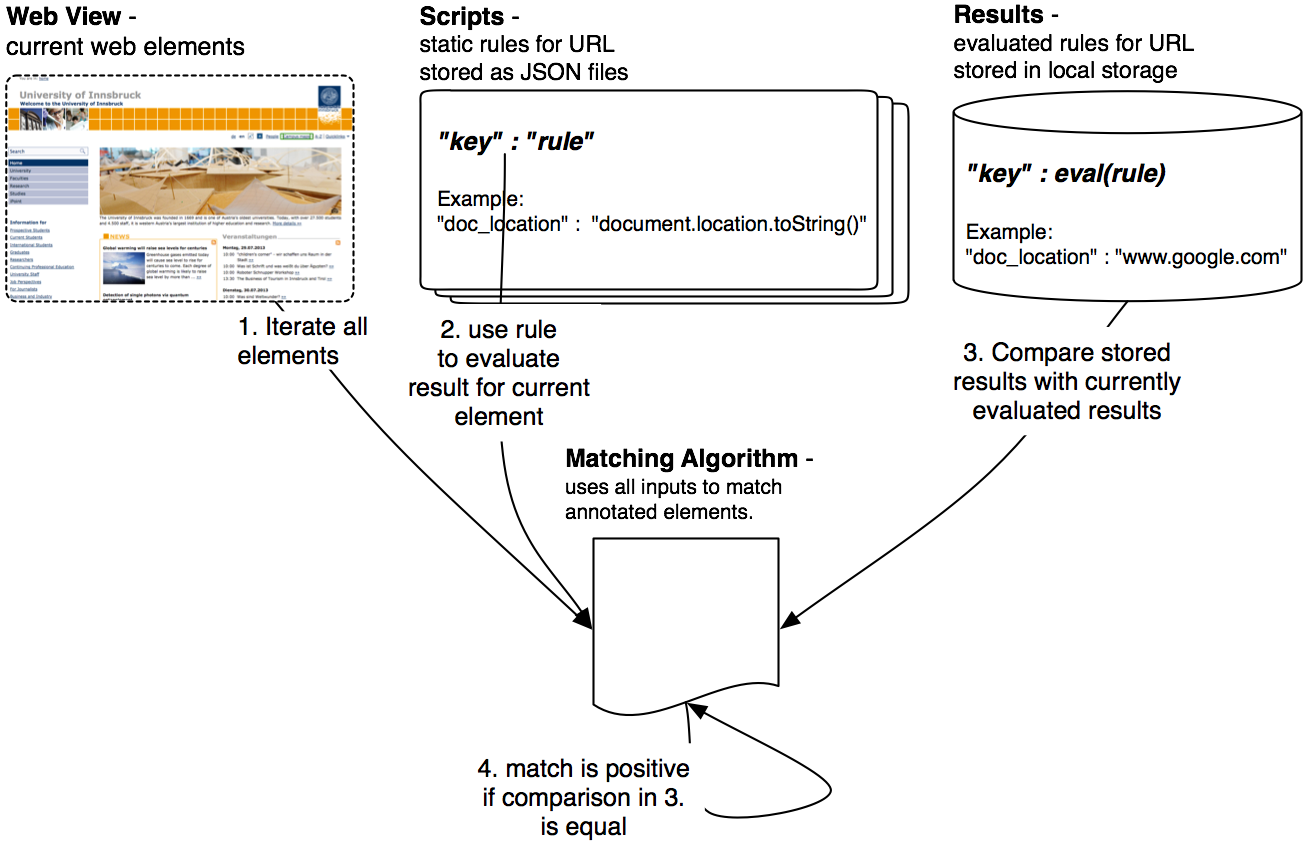
\includegraphics[width=13cm]{images/matching-algorithm.png}
\caption{Visualization for the different inputs for the matching algorithm}
\label{matching-algorithm}
\end{figure}

Once the matcher is triggered by opening a new web view the following algorithm take place:
\begin{lstlisting}
boolean positiveMatch = true;
for every element e in currentUrl{
	for every rule r in script.get(currentUrl){
		currentResult = r.execute(e);
		payloadResult = localStorage.getScript(currentUrl).getRuleResult(r);
		if(currentResult != payloadResult){
			positiveMatch = false;
			return;
		}
	}
}
\end{lstlisting}

Informally the algorithm iterates over every element in a new web view. This web view belongs to a certain URL that we use to determine what rule script to use. In case that no specific script is provided, a set of default rules is established. For every element, we execute the rules from the script and compare the results to possibly existing annotations. From the existing annotations, we store the evaluated rule results. Therefore, if an web element has the same results for all rule evaluations as an stored annotation, we assume that the current web element is an anchor that is related to the stored element. 

Since this issue is a little bit confusing, we explain what sources are used for decision making. See Figure \ref{matching-algorithm}. As sources for element matching, we have the current web view and all its displayed elements, the set of static rule contained by the scripts and the local storage that contains existing annotations. In the following every numbered step on Figure \ref{matching-algorithm} is explained in more detail:

\begin{enumerate}
\item We simply start with the mentioned iteration over all current web view elements. 

\item For each element all rules from the static script are executed. The results are stored temporarily just for the period of comparison in the next few steps.

\item Now need to check the temporary results from 2. according to the stored annotation data. If local storage contains a evaluated rule set that equals the temporary evaluation on the current web element, ...

\item ... then it is a match. 
\end{enumerate}

\paragraph{Algorithm Performance}
The above explained algorithms performance is not sufficient. The reason is the obvious $O(n^3)$ complexity due to the triple encapsulated for-loop. Since most web views have a quite limited amount of non-empty elements, it is no drawback for the prototype testing. However, it is easy to understand and to visualize. 
For reasons of completion, we look on a more efficient idea:
The basic problem is that we do not search for keys but values instead. In each step, we evaluate the value for the current web element and compare it to the values of all stored annotations. To overcome this issue, it would be necessary to generate hash values over all values of an element. 
For instance, an element that is identified with three rules gets a hash value generated from the composite of all rule results. Then this hash is used as the key of this annotation. 
This way we reduce the algorithm to a complexity of $O(n^2)$. The removed for-loop is the iterative search through stored annotations. This has become a hash search procedure that has the complexity of an average $O(1)$ and $O(n)$ in the worst case.

\newpage
\subsection{Social Weaver - Web Service}
The coming part is about the implementation of the web service that provides interfaces for our previously built plugin.

\subsection{Used Technologies}
Before we discuss our web service architecture, we first list the used technologies and give a brief explanation. Readers who are familiar with the following terms may skip this section. 
After pointing out the architecture, we map our defined requirements to our implementation and explain how those are achieved.

\begin{figure}\centering
		
\includegraphics[width=10cm]{images/ws-technologies-logos.png}
		\caption{Some of the used technologies for the web service}
		\label{ws-technologies-logos}
\end{figure} 

\subsubsection*{Model View Controller (MVC)}
The model view controller is the probably most common used user interface architecture pattern. Martin Fowler even writes in \cite{fowler2006gui} "I've lost count of the times I've seen something described as MVC which turned out to be nothing like it.". Since the reason, why we are applying MVC for our web service, is more a result of technology choosing, than an architectural one, there is need for explanation.

\begin{figure}\centering
		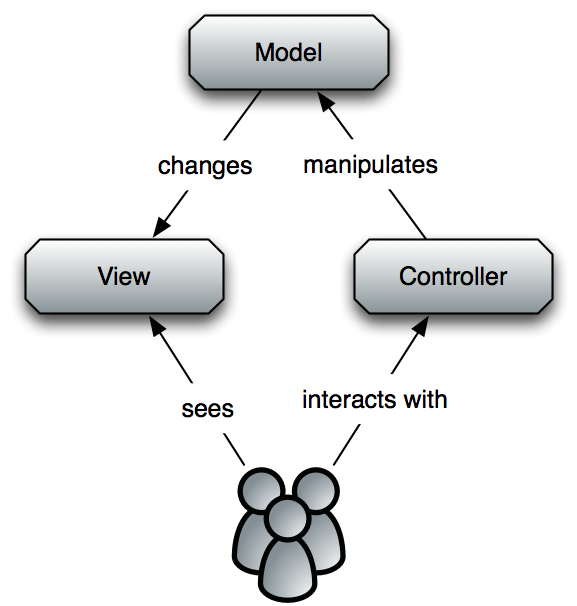
\includegraphics[width=8cm]{images/mvc-expl.png}
		\caption{Basic structure of MVC}
		\label{mvc-expl}
\end{figure} 


The basic idea of MVC is to separate displayed content and user interaction. As the name already reveals there are three modules that interact with each other and the user (also check Figure \ref{mvc-expl}):

\begin{description}
\item[Model] includes the logic of the system. That does not mean just business processes and functionality but even the persistence layer belongs to the model from the MVC perspective. 
The model updates the view and the controller manipulates the model.

\item[View] is the representation of some data. A view does not have to be a whole view in a browser (like it is when we use \emph{web view} outside this MVC context). It might represent a button, sub screen or any other user interface element.
The view is seen by the user and being updated by the model.

\item[Controller] takes input from user actions and use these to trigger operations included by the model. 
The controller manipulates the model and the user uses the controller.

\item[User] is able to see the content displayed by view and to use the controller parts to interact with the system. This is the essential part of MVC that seeing and interacting is separated. 
\end{description}

Even though our web service has a proper MVC architecture, we do not use it in the conventional way. Later we see that we use only RESTful requests to interact with the web service. It is easy and clean to extend a MVC pattern with additional interfaces for RESTful interactions. In addition, with certain technologies, like Spring Roo, it is faster to generate a classic web service.

\subsubsection*{OpenJPA}
OpenJPA is a object-relational mapping for the Java Persistence API (\sloppy \verb^javax.persistence^). The implementation makes it easier to interact with the persistence layer. Defining \verb^EntityManager^ for entities with some rules like

\begin{lstlisting}
public interface EntityManager {

    public void persist(Object entity);
    public <T> T merge(T entity);
    public void remove(Object entity);
    public <T> T find
		(Class<T> entityClass, 
			Object primaryKey);
    public <T> T find
		(Class<T> entityClass, 
			Object primaryKey, 
                	Map<String, Object> properties); 
    public <T> T find
		(Class<T> entityClass, 
			Object primaryKey,
                      	LockModeType lockMode);
	...
}
\end{lstlisting}
enables us to user persisted data nearly like objects. 
In the web service, any operation that writes to database is using OpenJPA.

\subsubsection*{PostgreSQL}
PostgreSQL is a cross-platform open source object-relational database system that the web service uses for the persistence layer. Since our database usage does not exceed basic operations there is no need to explain extended features of PostgreSQL.

\subsubsection*{RESTful Web Services}
RESTful web service or often-called RESTful web API as well use HTTP and REST principles. REST was defined the first time in Roy Fieldings doctoral dissertation \cite{fielding2000architectural}. It stands for \emph{representational state transfer}. REST uses the same types of operations as, for example, SOAP. These are:

\begin{enumerate}
\item GET
\item POST
\item PUT
\item PATCH
\item DELETE
\end{enumerate}

The central principle is that every accessible resource has its own and unique identifier (URI) in HTTP context. Related to this URI the different operations, mentioned above, can be executed. The RESTful provider handles each operation accordingly. We have two different cases where these operations slightly differ. It depends whether the URI belongs to a single resource entity (like for instance: \verb^http://localhost:8080/anchors/54^) or a set of entities (like \verb^http://localhost:8080/anchors^). Performing requests on a set, URI operates logically on sets. This means GET retrieves the whole list, POST adds a list of entities and DELETE deletes everything. On the contrary, requests on single resources only apply to the single element.  
	
\subsubsection*{Spring}
Spring is an application development framework for Java. Since its first release in 2002 it grew rapidly under the Apache 2.0 license \footnote{\url{http://www.apache.org/licenses/}} into several directions like modern web, data access, integration, mobile, social, security and cloud ready. All those sub frameworks provide different functionality. Besides that, there exist several side-projects. The web service makes use of one of those side-project that is called Spring Roo\footnote{\url{http://www.springsource.org/spring-roo}}. Roo is a development tool that makes it easy to create basic structures for web services with database connectivity. This tool makes extensive use of some Spring framework modules like Spring Integration, Spring Framework, Spring Security and Spring Web Flow. 
	
\subsubsection*{AspectJ}
	AspectJ is an extension to the Java programming language to provide aspect oriented programming. Even though AspectJ is the probably best-known representative for aspect orientation, the basic idea of this programming paradigm is applicable to any object oriented language.
	An aspect enables us to break down program logic to another layer. In object oriented environment most of the time the logic that is related to an object is included in the same class. With aspects, it becomes possible to distinguish different behaviors, related to an object, into different classes or even reuse them. 
	For instance, we have an entity controller for the anchor, the \textit{AnchorController}.This object is responsible for handling requests that arrive at the web service. Since there are several request types and different possibilities to answer them, we can distinguish between JSON and HTML requests. JSON requests can be sent by any client, whereas HTML is requested from the web client. We split those cases up into two separate aspect classes. By default these are called \textit{AnchorController\_Roo\_Controller} and \textit{AnchorController\_Roo\_Json}. 
	Using aspects becomes more valuable with increasing complexity. The \textit{Anchor} entity is split into aspects for bean-, JPA entity-, JSON-functionality etc.

\newpage
\subsection{Web Service Architecture}\label{ws-architecture-intro}
The web service is a common MVC architecture that uses JSON/RESTful interfaces. The persistence layer is connected to a PostgreSQL database using OpenJPA. 

Our main entities are the anchor and social element. The anchor has been already discussed from the concept point of view. The entity contains all the parameters that are necessary for matching web elements. This set of parameters can differ from one web application to another. Additionally the anchor entity contains a unique object identifier (OID) that defines the anchor even across different user sessions. This way updates can be performed more easily without having to check for all parameters every time. Which would be hard especially in those cases where an unusual set of matching parameters is being used. To avoid this difficulty but to still keep all parameters related we generate a hash from a combination of all relevant parameters. This hash is used as OID. 
Besides that the Anchor holds a time stamp with information about the last modified date. We use this data for the synchronization procedure. 

The social element entity is handled as a separate entity but from the concept perspective, it is a part of the Anchor. It works as a container for any kind of social content. Because our prototype just provides a simple HTML inject, the social element contains an URL and a reference to the Anchor. Nevertheless, it is extendable to hold data for native and more complex social element types. 

The entities are implemented as beans and therefore being directly persisted in the PostgreSQL database.

According to the model view controller pattern, there are also controllers for the entities that provide several interfaces that are accessible through the standard REST requests. 

\begin{figure}\centering
		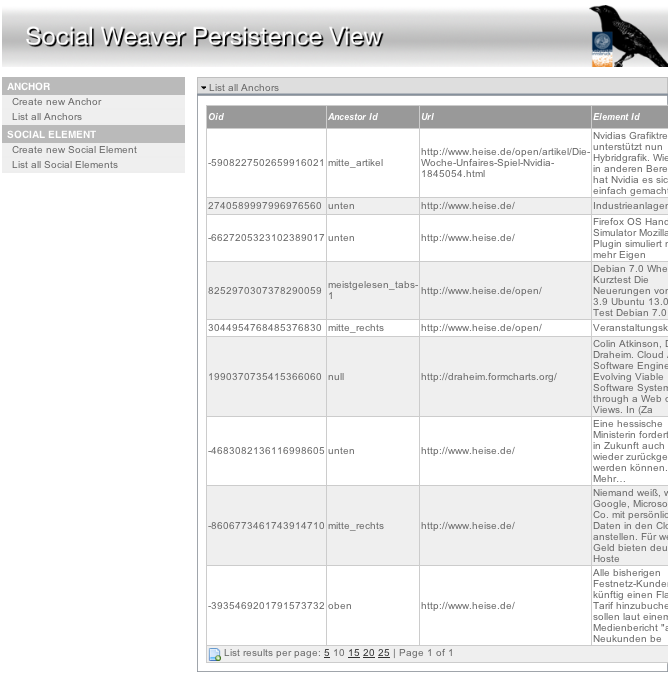
\includegraphics[width=7cm]{images/sowe-mvc-view-screenshot.png}
		\caption{Screen shot from Social Weaver Persistence Web View}
		\label{sowe-mvc-view-screenshot}
\end{figure} 

The View from our Model View Controller architecture is a web view that allows the user to check the content manually (see Figure \ref{sowe-mvc-view-screenshot}). This is just a pleasant side feature and not related to our Social Weaving use cases and for that reason this part should be discussed no further.

\newpage
\subsection{Requirements for the Web Service}
In Section \ref{Social Weaver - Server Application} we defined the following requirements for the web service:

\begin{enumerate}
\item \reqWSi
\item \reqWSii
\item \reqWSiii
\item \reqWSiv
\item \reqWSv
\item \reqWSvi
\item \reqWSvii
\end{enumerate}

In the following, we explain requirement by requirement how the prototype web service implements the features. The introduction of \ref{ws-architecture-intro} included a brief overview of the web service. Technical details only are shown and discussed when relevant to the fulfillment of the corresponding requirement.

\subsubsection[Incoming Messages]{\reqWSi}

For the needs of the prototype, we use a standard RESTful PUT interface on the server side for the anchor entity:

\begin{lstlisting}[language=Java]
{
    @RequestMapping(method = RequestMethod.PUT, headers = "Accept=application/json")
    public ResponseEntity<String> AnchorController.updateFromJson(@RequestBody String json) {
        HttpHeaders headers = new HttpHeaders();
        headers.add("Content-Type", "application/json");
        Anchor anchor = Anchor.fromJsonToAnchor(json);
        if (anchor.merge() == null) {
            return new ResponseEntity<String>(headers, HttpStatus.NOT_FOUND);
        }
        return new ResponseEntity<String>(headers, HttpStatus.OK);
    }
\end{lstlisting}

With no security restrictions, any client can send a request and since the anchor format is valid, the web service persists the data into the database. The request body has to have JSON format. The JSON body is deserialized (line five) using the default JSONDeserializer provided by the Flexjson framework\footnote{\url{http://flexjson.sourceforge.net/}}. The fact that we use a PUT request enables us to either update or create new entities. Messages that have the same payload create the same OID hash. Every anchor on the same element is recognized as an update. New anchors insert a new entity. 

A possible and valid PUT request using cURL\footnote{\url{http://curl.haxx.se/}} could look like:

\begin{verbatim}
curl -i -H "Accept: application/json" -X PUT -d 
"url='http://draheim.formcharts.org/', 
payload='[
	{"doc_location":"http://draheim.formcharts.org/"},
	{"element_content":"PD Dr. Dirk Draheim"}
]'"  
http://localhost:8080/anchors
\end{verbatim}

This way of receiving requests is very simple and provides no handling for user sessions, secure authentication or validation of anchors.

\subsubsection[User Session Synchronization]{\reqWSii}

The prototype does not provide specific user sessions. This would be desirable as an extended feature. The web service handles synchronization between different users exactly as for one user. 
Any message with an anchor that is received, injects into the data set of anchors. We use a time stamp to signalize that updates were made. When users synchronize with the server the simply receive all anchors that are newer than the newest anchor located in the users plugin. 

We clarify this on a small use case scenario with Alice and Bob:
\begin{enumerate}
\item Alice starts the plugin and synchronizes at time n. It is a new session so no anchors are sent back to Alice. Both parties, Alice and the web service, have n set as update time stamp.
\item Alice adds two anchors to the data set. These anchors transmit to the server and get the time stamp n+1.
\item Alice automatically synchronizes with the server after sending the update. Again, both parties have a synchronized time stamp (n+1).
\item Bob joins this session and start his plugin. This initiates synchronization and Bob gets all updates until n+1.
\item Bob sends a new anchor to the server. 
\item The web services receives the anchor and sets its time stamp to n+2. 
\item Bob automatically synchronizes his local data content. Bob and the web service are now at time stamp n+2. 
\item Alice has to refresh the plugin since the server is silent. Until Alice or the plugin initiate synchronization, Alice keeps time stamp n+1
\end{enumerate}

Besides the drawbacks that users cannot determine who made what changes (and when), the web service has the issue that no push notifications are supported. The plugin is regularly update automatically or triggered by specific actions. Such actions can be update requests or opening new web views. 

\begin{figure}\centering
		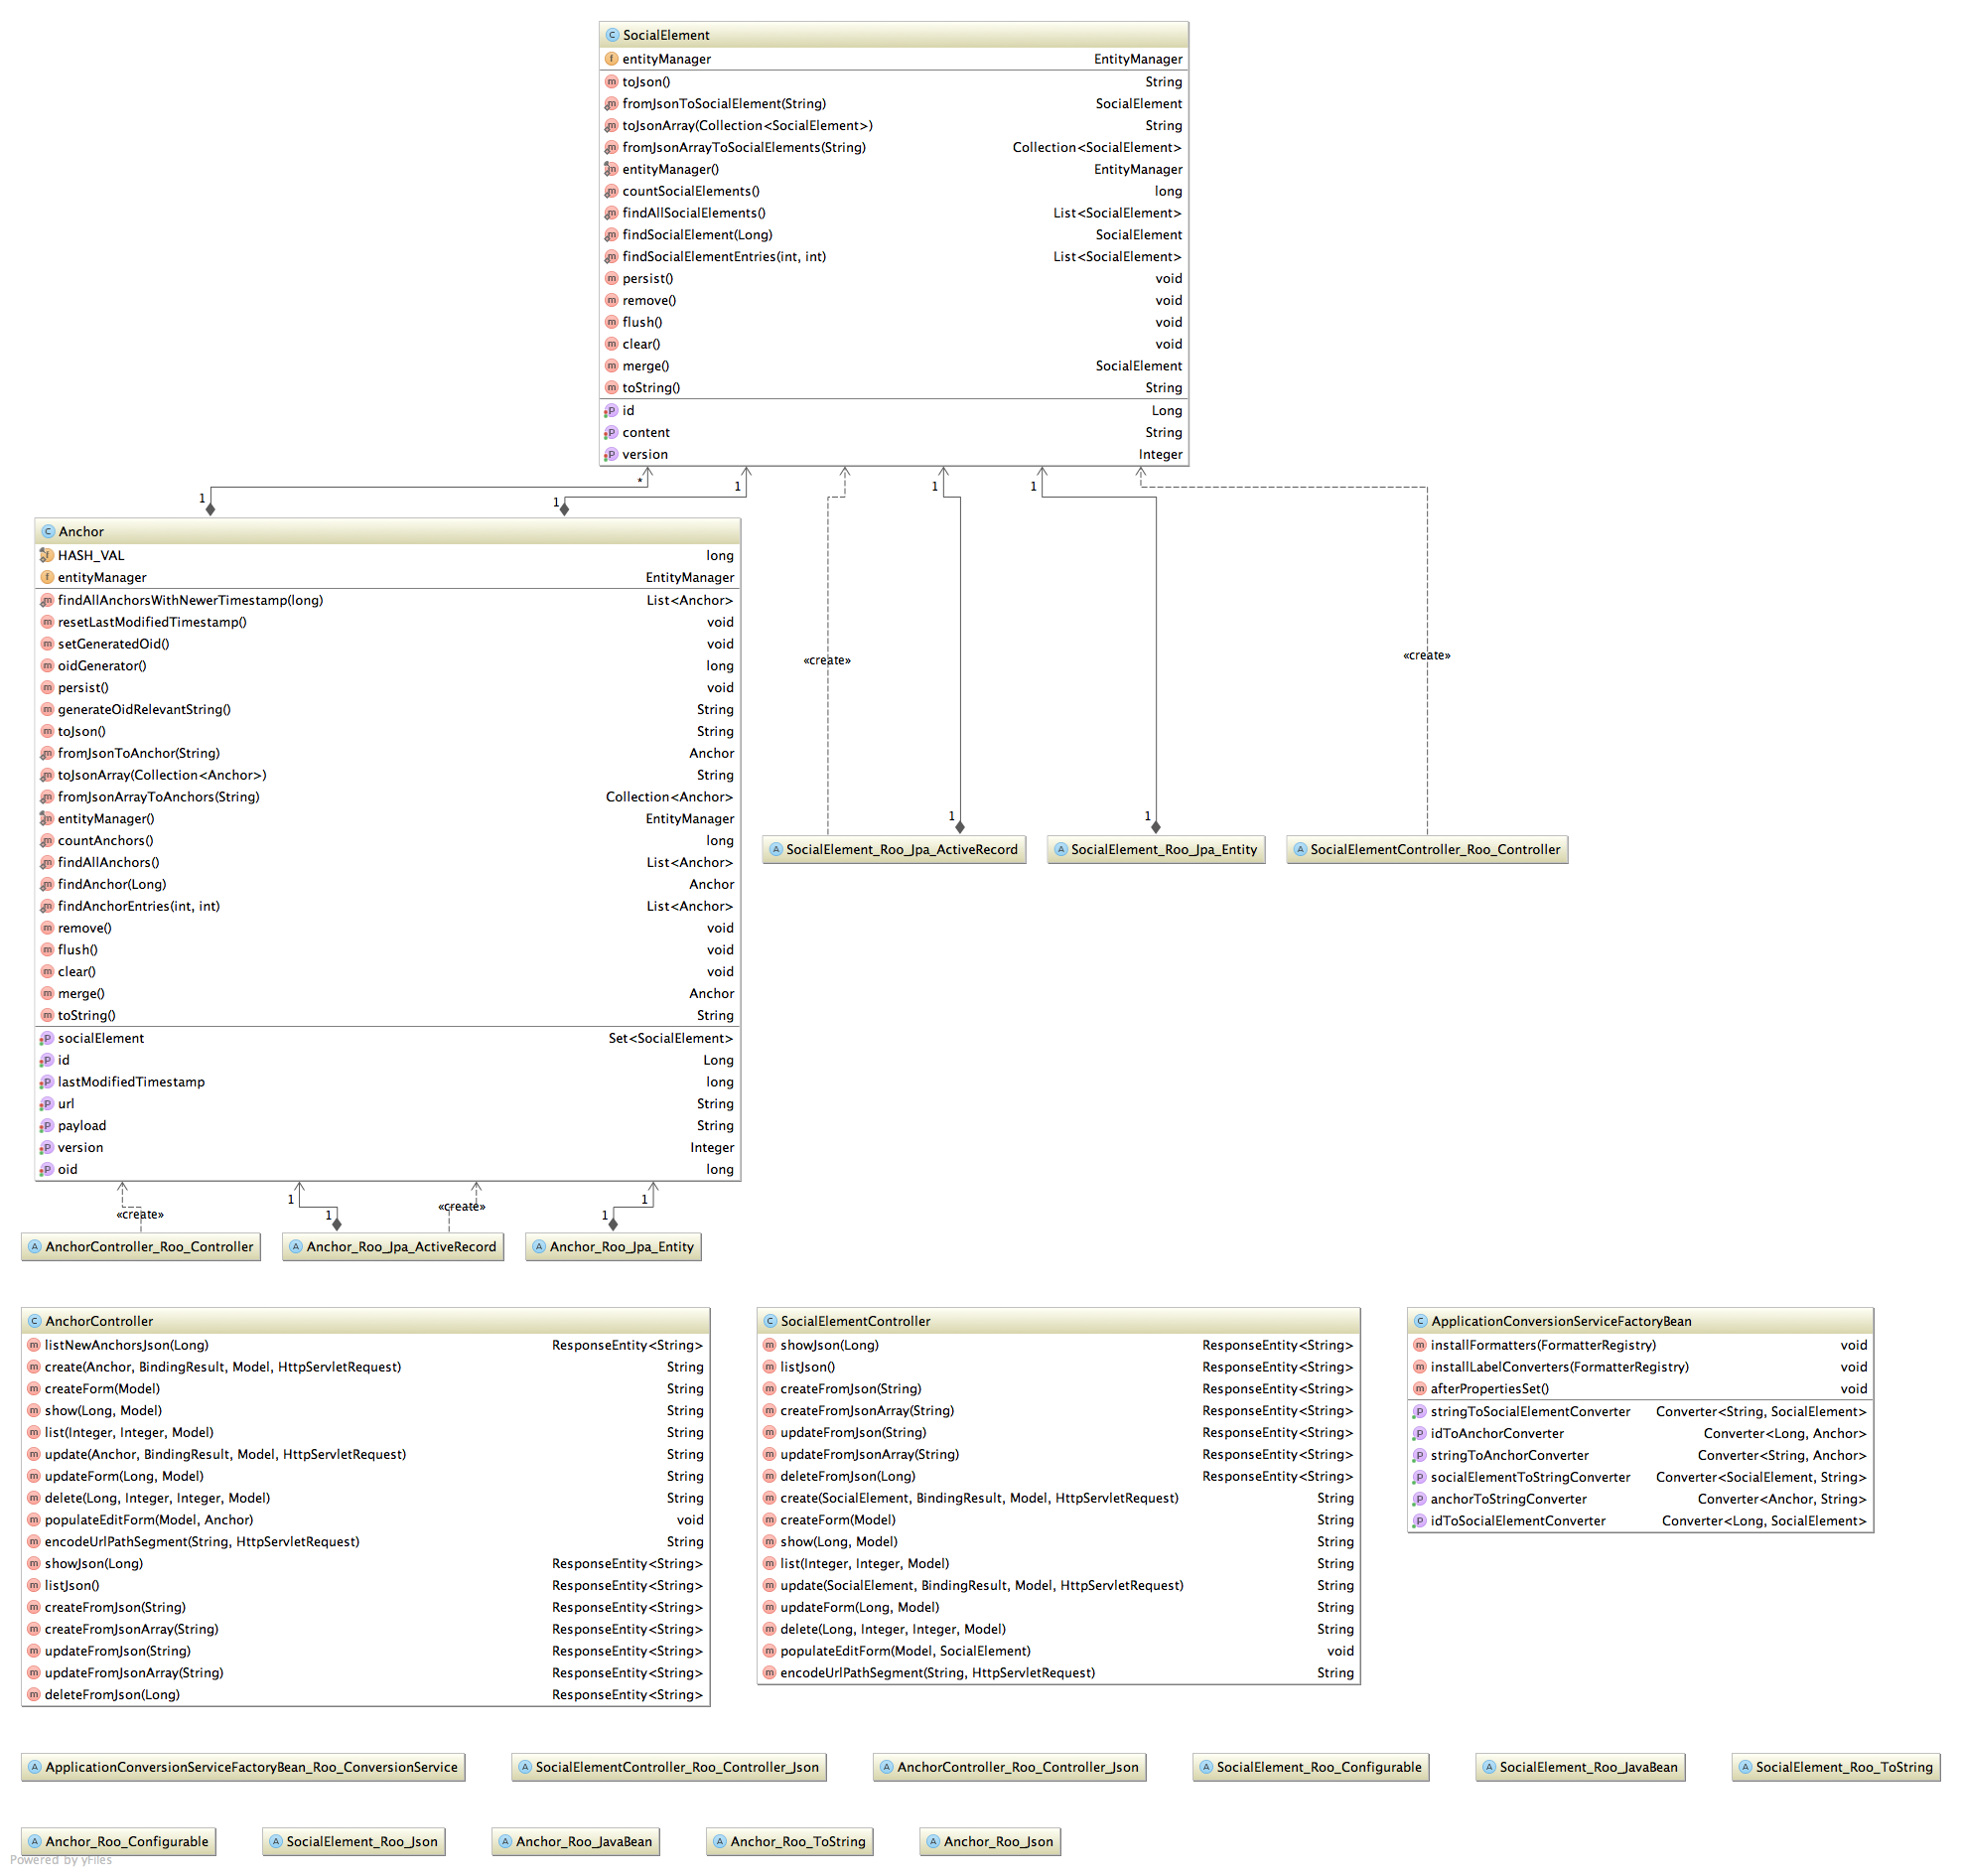
\includegraphics[width=13cm]{images/sowe-ws-uml-package.png}
		\caption{UML package diagram from web service}
		\label{sowe-ws-uml-package}
\end{figure} 

This minimalistic user synchronization support is sufficient for showing how Social Weaving works across different hosts though.

\subsubsection[Persistence]{\reqWSiii}
Once the REST service receives and deserializes the JSON file, we proceed with populating the new data into the database. Since we use PUT functionality we need to merge it eventually into already existing database entries. This is realized using the following implementation:

\begin{lstlisting}[language=Java]
{
    @Transactional
    public Anchor Anchor.merge() {
        if (this.entityManager == null) this.entityManager = entityManager();
        Anchor merged = this.entityManager.merge(this);
        this.entityManager.flush();
        return merged;
    }
}
\end{lstlisting}

As entity manager we use the standard from the \verb^javax.persistence^ library\footnote{\url{http://docs.oracle.com/javaee/6/api/javax/persistence/package-summary.html}}. The entity manager is configured with OpenJPA and connected to a PostgreSQL database. 

\begin{figure}
	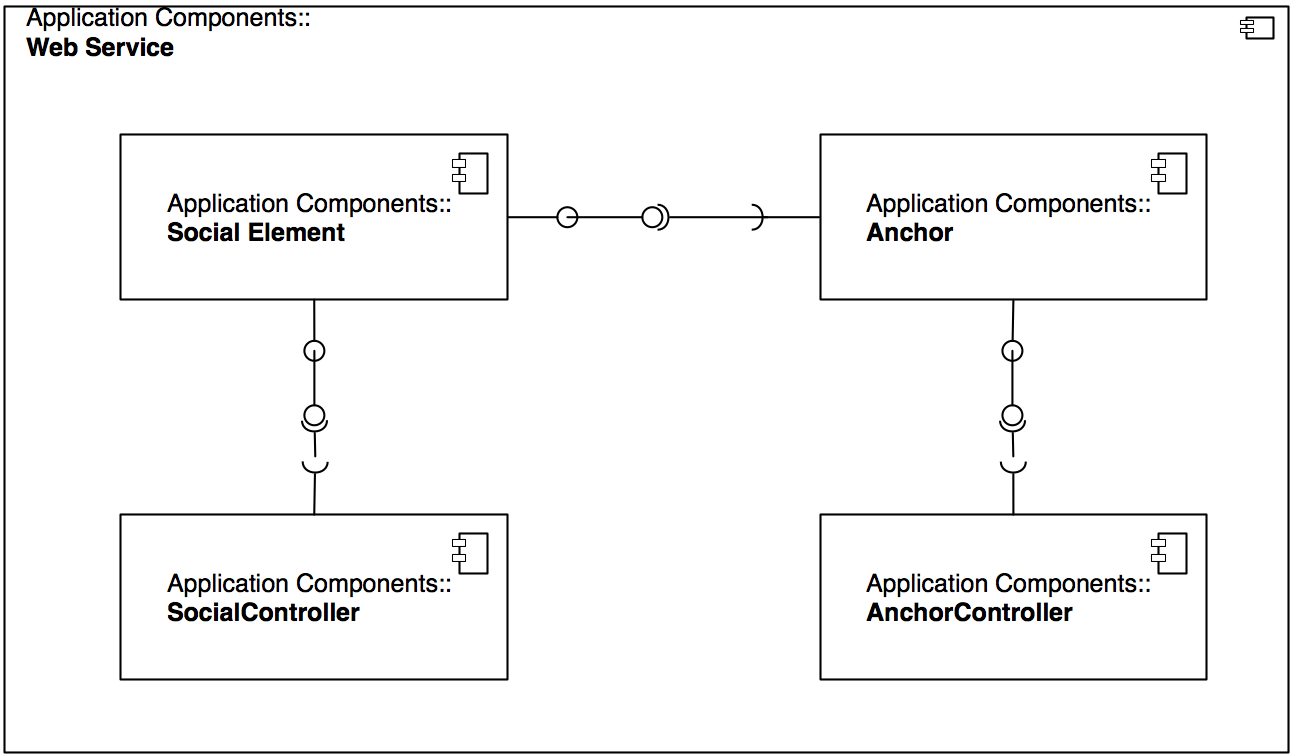
\includegraphics[width=13cm]{images/component-server-diagram.png}
	\caption{Component diagram for the web service}
	\label{component-server-diagram}
\end{figure}

\subsubsection[Decoupling Web Service and Target Web View]{\reqWSiv}\label{reqWSiv}
In the decoupling requirement, it is about the content of the annotation messages that are transmitted between plugin and web service. The requirement should ensure that the message form is independent from the target web view. The target web view is the web page or application the annotation belongs to. 
The web service needs to be able to synchronize all annotations simultaneously no matter where they are annotated. For instance, one annotation made on \url{http://www.uibk.ac.at/} has the same form and is handled equally as an annotation from \url{internal-sap.examplecoorp:4567}. 

To affirm that this constraint is not disturbed, messages are handled as information containers. Once they arrive at the web service, it provides those without any knowledge about the inside of the message. All operations on the data is read-only. 

\subsubsection[Decoupling Web Service and Plugin]{\reqWSv}\label{reqWSv}

The previous decoupling requirement \ref{reqWSiv} was about the content of messages. This requirement is about the message format and the processing rules. Since the Social Weaver prototype provides a plugin for Firefox only, this requirement is more a heads-up for potential upcoming development of plugins for other browsers. 
The exact format of the messages has been discussed already in the context of plugin requirements (\ref{reqPv} and \ref{reqPvi}) and is issue in the coming Sections (\ref{reqWSvi} and \ref{reqWSvii}). As long this format is kept up, the requirement fulfillment remains valid. 

\subsubsection[Message Parsing]{\reqWSvi}\label{reqWSvi}

Formerly message parsing was discussed in Section \ref{reqPvi}. Hence this section does not cover the way of creating the message. We just assume the defined format, which was:
\begin{lstlisting}
{"annotation":[
	 {"url": "http://www.uibk.ac.at/"},
	 {"payload":[
 			{"doc_location":"http://www.uibk.ac.at/"},
 			{"element_content":"Campus maps"}
 	]},
 	{"social_element":"http://www.uibk.ac.at/internalwiki/faqs"}
 ]}
\end{lstlisting}

In Section \ref{reqWSv} we stated that the web service does not modify the content of the message. The only operations are read only. The following steps take place when a new annotation array arrives:

\begin{enumerate}
	\item The array is split and the annotations handled separately 
	\item Each annotation is split into its elements: \verb^url, payload^ and \verb^social_element^
	\item \verb^url^ and \verb^payload^ are stored as values in an anchor entity
	\item \verb^social_element^ is stored as value in a social element entity
	\item Each time an anchor is persisted it updates its time stamp to the most recent update time
	\item The primary key for an anchor becomes a has value over the payload and url
\end{enumerate}

It is possible that an incoming annotation already exists and therefore is just an update. This case only differs slightly from the procedure mentioned above. The \verb^social_element^ is overwritten with the new content. The anchor entity receives an up to date time stamp. However, the remaining fields remain untouched. 

\subsubsection[Generating Messages]{\reqWSvii}\label{reqWSvii}
Generating outgoing messages in this context means providing them as JSON representation through a RESTful interface. There are several interface for retrieving annotations from the web service like:
\begin{lstlisting}
@RequestMapping(headers = "Accept=application/json")
    @ResponseBody
    public ResponseEntity<String> AnchorController.listJson() {
        HttpHeaders headers = new HttpHeaders();
        headers.add("Content-Type", "application/json; charset=utf-8");
        List<Anchor> result = Anchor.findAllAnchors();
        return new ResponseEntity<String>(Anchor.toJsonArray(result), headers, HttpStatus.OK);
    }
\end{lstlisting}
It is possible as well to retrieve specific annotations by its value or key. Most of the time, we need the special query for retrieving only the newest anchors. This task is accomplished by:

\begin{lstlisting}
@RequestMapping(value="/updates/{lastModifiedTimestamp}")
    public ResponseEntity<String> listNewAnchorsJson(@PathVariable Long lastModifiedTimestamp) {
        HttpHeaders headers = new HttpHeaders();
        headers.add("Content-Type", "application/json; charset=utf-8");
        List<Anchor> result = Anchor.findAllAnchorsWithNewerTimestamp(lastModifiedTimestamp);
        return new ResponseEntity<String>(Anchor.toJsonArray(result), headers, HttpStatus.OK);
    }
\end{lstlisting}

Since these methods are formed according to the spring standard, the only part that requires explanation is the actual \verb^finder^ method in line five. Behind the scenes we use a \verb^TypedQuery^ (Figure. \ref{typed-query}) to create a modified SQL query that returns all entities that has a newer time stamp than the parameter, that has been passed from the plugin.

\begin{figure}\centering
\begin{lstlisting}
TypedQuery<Anchor> query = entityManager().createQuery("SELECT o FROM Anchor o WHERE o.lastModifiedTimestamp > :ts", Anchor.class);
\end{lstlisting}
\label{typed-query}
\end{figure} 

\newpage
\subsection{Social Weaver - Script Support}\label{sowe-script-support}
The following part explains how the script support looks like in detail for our Firefox plugin. In Section \ref{abstract-script-support-reqs} we discussed the purpose of the script support and what its goals are. The coming part applies this knowledge practically to the prototype development. Before we start stepping through the gathered requirements from \ref{abstract-script-support-reqs}, a brief example of a script use case is explained to provide a better overview to the reader.

A script contains the information about how an element in a web view might be found. We use JSON as format for the scripts because of the support that JavaScript provides for that standard. The script defines a set of rules that are used to perform operations on the selected element. The results from these operations are generated to a payload. This payload might be the information for anchors, URL and content related to social elements. The server handles this payload as one value and does not parse it. All Meta information that are needed by the server are transmitted separately from it. To understand how the script is used to generate an anchor format, we look at the example:

\begin{lstlisting}
{
    rules:
    [

         {"doc_location" : "document.location.toString()"},
         {"element_content" : "$(matchedElement).text()"},
         {"element_children" : "$(matchedElement).children().text()"},
         {"element_content": "matchedElement.innerHTML"},
         {"dom_path": "true"}	
    ]
}
\end{lstlisting}

The purpose of this script example is to show the different possibilities and not a real scenario use case. It becomes obvious why this set of parameters would be no good choice. 

A script is a set of rules. A rule consists of a key name and the actual operation that is being used to perform an action. The key name can be any string within quotes chosen by the script author. The key names should be unique in one script though. The operation part offers different opportunities:

\begin{itemize}
	\item jQuery Operation \\ 
	jQuery is a great possibility to traverse the DOM tree and it is possible to inject jQuery commands directly in the script. It is necessary that the command return a string that is used for identification. The first line
		\begin{lstlisting}
		         {"doc_location" : "document.location.toString()"}
		\end{lstlisting}
	would tell the plugin to save the document location - which is the plain URL in most cases. 
	
	To trigger an operation related to the element that has been clicked by the user we might use the keyword \verb^matchedElement^. In case a jQuery method is used, it is still necessary to transform the matched element to jQuery format (\verb^matchedElement^ $\rightarrow$ \verb^$(matchedElement)^). 
	
	\item	 JavaScript Operation \\
	Even though most functionality related to DOM tree traversing should be covered with jQuery it might be of use sometimes to use JavaScript commands directly. 
		\begin{lstlisting}
		         {"element_content": "matchedElement.innerHTML"}
		\end{lstlisting}
	This line is an example for how to retrieve the HTML content of an element. This information might be used for matching elements for instance. 
	
	\item Predefined Operation \label{predefined-operation}\\
	Some functions we need are not directly provided using JavaScript. The best example for such a case is the DOM tree path. We can use the DOM tree path for distinguishing similar elements. This functionality is provided by the plugin and can be enabled or disabled with the rule:
		\begin{lstlisting}
		         {"dom_path": "true"}
		\end{lstlisting}	
\end{itemize}

\subsection{Requirements for the Script Support}

In the conceptual Section \ref{abstract-script-support-reqs} we defined a couple of abstract requirements that we need to specify for a proper implementation. Those requirements were:

\begin{enumerate}
\item \reqSi
\item \reqSii
\item \reqSiii
\item \reqSiv
\item \reqSv
\item \reqSvi
\end{enumerate}

\subsubsection[Information Container]{\reqSi}

For matching different elements, we need the flexibility to use a variable set of rules. It would be a drawback to have a static rule system. The problem is that in some web views we need different operations to match elements than on others. Depending on the environment, we need a specific container with the rule set. 

We solve this issue by introducing the payload container that contains a JSON array with all information that is set by the script. This way we are able to extend information for element matching and modify it just by changing the script. The plugin and backbone of our system does not necessarily have to be changed because it always is handled as a single JSON string.

\subsubsection[Decoupling]{\reqSii}\label{decoupled-req}

The script itself does not contain any information of the browser plugin type or the server module. The defined rules need to be supported by the plugin though. 

A plugin that does not support jQuery commands would not work with our script example from above. Or the \emph{predefined operation} (mentioned in \ref{predefined-operation}) is another case that needs to be supported by the plugin. Using unknown or unsupported operations leads to unexpected results.  

The server on the other hand is completely decoupled from the script support. The payload is just one column and the information about element anchors is of no use for the server. This is way the payload is not be parsed on the server. 

Even corrupt payloads that cannot be used by the plugin are perfectly synchronized at the back end. This might seem not much of use at first appearance. Nevertheless, there is the case when a the payload for matching an element becomes defect not by using wrong rules, but because of some changes in the web view. Then we still want to keep the information about the element and just re-create the payload to it. Hence, it makes sense to keep even those elements in the server database.

\subsubsection[Syntax]{\reqSiii}

It is a desirable goal for the future to have a system, like a script generator, that can be used be persons without any technical knowledge. However, since we conduct prototype development we at least assume knowledge about web development. To choose the right rules and operations for element matching requires this kind of knowledge anyway. 

JSON is commonly used format and even possible to read by persons without technical knowledge. When providing a template with some example rules it is obvious to see how these rules might be extended. 
The most challenging part is to find and define the correct set of rules - but this is beyond the scope. 

Beyond the criterion, that scripts are human-readable it would be easy to create a form or generator with a graphical interface to generate such scripts. Error handling could be supported already at this point. Even more desirable is an automatic script generator that generates scripts from user behavior without his active interaction (or at least minimal). 

\subsubsection[Plugin Extension]{\reqSiv}

When we were talking about rules and operations for element matching, this included short Java Script or jQuery commands. Technically, we are not limited to short commands and it is possible to insert a whole command block as a rule. Nevertheless, for debugging reasons this is not a good solution. Moreover, some operations may require more than just a chain of jQuery commands. 

For example, we take the procedure of determining the DOM path of an element in the tree. The idea is to start with the class name of the element itself. Then check the class name of its parents so long until the root of the DOM tree is reached. All names chained together describe the path of the element in the tree. The fact that this result is not necessarily unique underlies the problem that DOM trees are often ambiguous. We take a closer look on this issue in \ref{ambiguity-problem} \nameref{ambiguity-problem}. However, for some web views the DOM path still might be the right choice. 

To understand why such a procedure is not possible to be fitted in a script we need to look at the code first:

\begin{lstlisting}[language=JavaScript]
    var rightArrowParents = [];

    $(this).parents().not('html').each(function() {
        var entry = this.tagName.toLowerCase();

        if (this.className) {
            entry += "." + this.className.replace(/ /g, '.');
        }

        rightArrowParents.push(entry);
    });
    rightArrowParents.reverse();    
    var domPath = rightArrowParents.join(";");
\end{lstlisting}

In line three we initiate a loop for all parent elements of the selected element \verb^this^. We watch out for every parent that has a \verb^className^ in line six. In a positive case, we add this information to our path result. 

The problem why we cannot insert such an operation into a script is, that we need an outside variable for keeping track of the results through the loop iterations. Line three until eleven is the actual jQuery command. Nevertheless, it would be a mess to pass the whole code with the script. Theoretically, it would be possible to support such scripts but it would make the script idea even more error prone. 

Instead we use \emph{predefined functions}. Those functions are implemented directly in the plugin and can be triggered using defined rules in the script. 

To enable the DOM path parameter in the rule set we would just need to insert this rule:
\begin{lstlisting}
         {"dom_path": "true"}
\end{lstlisting}
The plugin would recognize this rule and run the code that determines the DOM path. In the Section \ref{decoupled-req} we already mentioned that this way of supporting more complex operations leads to minor coupling between plugin and script. 

\subsubsection[Default Matching Procedure]{\reqSv}\label{reqSv}

Even though it is not possible to provide a default matching algorithm that applies to any web view, it is desirable to at least have some default matching in case to specific script for the visited URL exists. If the user visits a new environment, there is at least the chance that some elements might be matched.

To fulfill this requirement, the plugin provides a default script. When a new web view is loaded - all scripts are checked whether one of them applies to the new page. If it is not the case, the default script is chosen and the user notified. 

\subsubsection[Relation to URL set]{\reqSvi}

Every script, except for the default script from \ref{reqSv}, mostly needs to be related to a specific environment. When we talk about environment in this case, it means views that inherit from a root URL. As example a script can be related to \url{http://www.gnu.org}. But any page that has this URL as root, like, for instance, \url{http://www.gnu.org/philosophy/philosophy.html}, still applies to the same script. 

The assumption is that views in the same environment apply to the same web architecture and hence its elements can be identified similarly. 

Obviously, this must not hold for every case. A web view can have a very different architecture than its root. Nevertheless, for prototype development this drawback is considered as tolerable. 

\newpage
\subsection{Ambiguity Problem}\label{ambiguity-problem}

Throughout the conceptual (\ref{sowe-abstract}) and implementation (\ref{sowe-concrete}) section about the prototype development we often noticed issues that make it tricky to achieve the proposed goals. The greatest challenge by far is the unique recognition of elements in a web view. More precisely: the finding of an element in the DOM tree. 

This procedure consists of the two steps:
\begin{enumerate}
	\item User chooses element from view
	\item Plugin searches for this element from the DOM tree
\end{enumerate}

The first step is easy because we have the clear information from the user input. The hard work is done by the user. Still our problematic situation takes place already at this point. 

Hence the plugin needs to know in what way it is going to identify the element in the second step, it is necessary to gather all the information in first step. This is were the rules from a script (\ref{sowe-script-support}) come in. Those rules are commands that are executed and retrieve results. Those results identify the element. 

In the second step, when a view is opened, all appearing elements are checked with the script rules and the results compared to our results from step one. If the results appear to be the same - we assume it is the searched element. 

The fact that we can only assume, finally leads us to the actual problem of this section. The DOM tree can be ambiguous and in fact, this is no exception.

\subsubsection{Ambiguous Grammar}
\begin{figure}\centering
		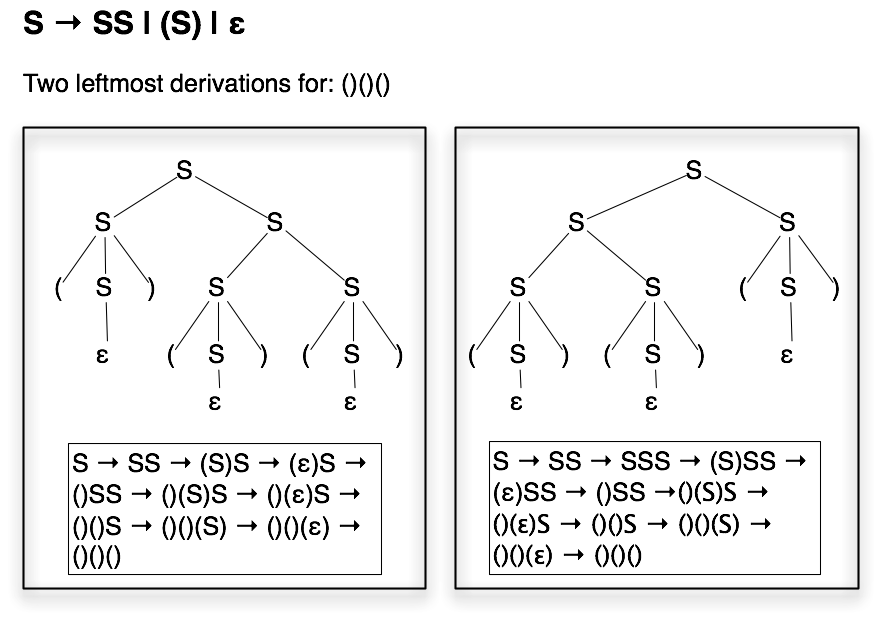
\includegraphics[width=10cm]{images/ambiguous-grammar.png}
		\caption{Example for an ambiguous grammar}
		\label{ambiguous-grammar-pic}
\end{figure} 

We know the origin of ambiguity in computer science from formal grammars. A grammar is ambiguous for which there exists a string that has more than one leftmost derivation. Check Figure \ref{ambiguous-grammar-pic} for a common example of a ambiguous grammar.
\begin{lstlisting}[mathescape]
S $\rightarrow$ SS | (S) | $\epsilon$
\end{lstlisting}
This generates a chain of correct opening and closing brackets. The grammar is ambiguous because we have to ways of generating the same string \verb^()()()^. For the parse tree and step by step creation see again the Figure \ref{ambiguous-grammar-pic}.

\subsubsection{Ambiguity for Element Matching}

What is the concern of ambiguous grammars when we talk about web architectures? We use the basic idea of ambiguity to describe the problem giving elements unique parameters. Imagine we would try to identify elements just on their location in the DOM tree. At a first glance this may appear as an effective way since we are used to storing data in tree based data structures. 

We explain the problem with the HTML example in Figure \ref{dom-html-example}.

\begin{figure}
\begin{lstlisting}
<html>
	<head>
			<title>Software Development</title>
	</head>
	<body>
		<b>Software Development Activities</b>
		<ul>		
			<li> Requirements 
			<li> Construction 
			<li> Deploying		
		</ul>
		<b>Software Development Methodologies</b>
		<ul>		
			<li> Spiral
			<li> V-Model 
			<li> Scrum		
		</ul>
	</body>
</html>
\end{lstlisting}
\label{dom-html-example}
\caption{HTML example for showing ambiguity}
\end{figure}


\begin{figure}\centering
		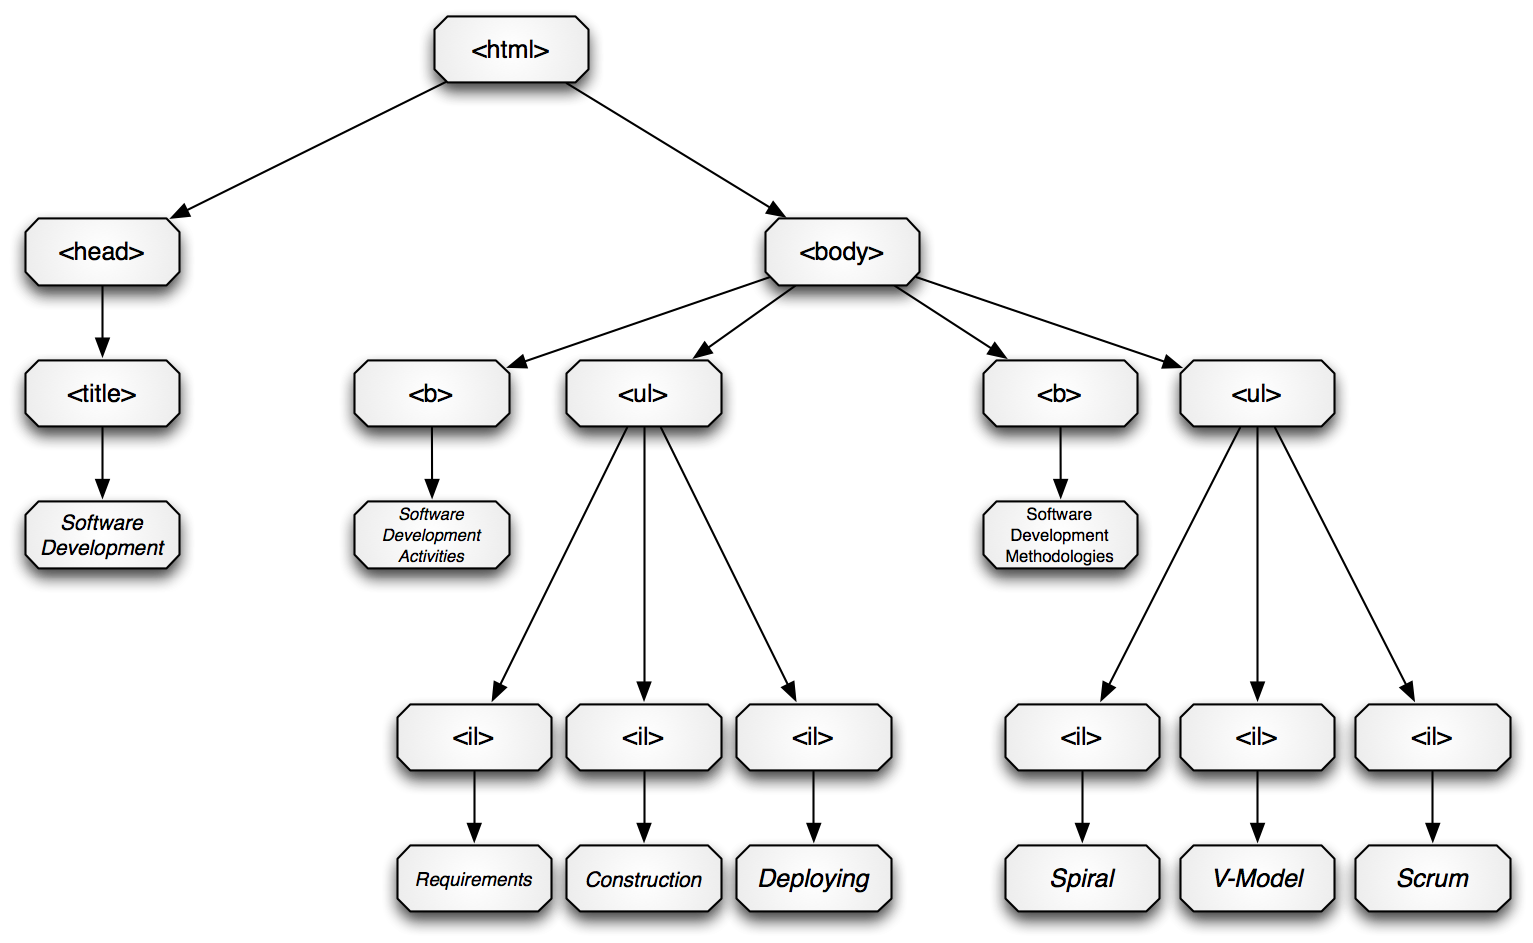
\includegraphics[width=13cm]{images/dom-tree-example.png}
		\caption{DOM tree representation for HTML code in Figure \ref{dom-html-example}}
		\label{dom-tree-example}
\end{figure} 

Determining the DOM path for \verb^Software Development^ would return the value: \verb^<html>,<head>,<title>^. In this case, the path would be a unique identifier in this environment. 
The DOM path for \verb^Construction^ would be \verb^<html>,<body>,<ul>,<li>^. This path would not only apply to all \verb^<li>^ elements in the same \verb^<ul>^ context, but to all \verb^<ul>^ lists in the same sub path (which is \verb^<html>,<body>^ so far). Using this path would apply to all six list elements. 

\subsubsection{Parameter Data Object Model Tree}\label{param-dom-tree}

For the moment we forget that we can use other parameters (like the \verb^<li>^ content or surrounding parameters like the \verb^<b>^ blocks to identify elements. 
When we represent the HTML code as DOM tree, we receive a structure where it seems that every element can be located uniquely (see Figure \ref{dom-tree-example}). The parameter DOM path for \verb^Construction^, which has the regular DOM path \verb^<html>,<body>,<ul>,<li>^, would become \verb^#0<html>,#0<body>,#0<ul>,#1<li>^. 
To keep that feature available in-code, we need to create a copy of the actual DOM tree and add parameters that uniquely identify the class types. 
The parameters are set by following the algorithm in Figure \ref{alg-param-dom-tree}. Informally this algorithm starts at the root and marks it. From there on every child is classified for its class type. Children with the same class type are marked with an incremental counter. This operation is recursively be repeated until no child has a class type. 
Applying this algorithm to the DOM tree in Figure \ref{dom-tree-example} we receive the parameter DOM tree in Figure \ref{dom-paramaterized-tree-example}. As you can see the class type \verb^<b>^ is marked with \verb^#0^ as well as \verb^<ul>^. Even though both children have the same parent, there is no need to use the same counter for marking.

\begin{figure}
\begin{description}
	\item[1] Select the root as current node and mark it with \#0
	\item[2] Retrieve class types of all children
	\item[3] Mark every class type set with an incremental counter starting with \#0 to \#n
	\item[4] Repeat Steps two and three for every child until no child has class type
\end{description}
\caption{Algorithm for parameter DOM tree}
\label{alg-param-dom-tree}
\end{figure}

The advantage of using increment for same class types only is a better robustness. If the HTML code change it might happen that the parameter DOM tree becomes corrupt. With independent counters, impacts from changes are attenuated. 
The idea of the parameter DOM tree is just mentioned for reasons of completeness. The algorithm is not implemented in the prototype because of practical reasons. 

The parameter DOM path is more effective than the regular path, because it overcomes the ambiguity problem. But there still are problem that apply to both methods. Web applications and pages changes frequently and though the underlying HTML code. When we use the a tree representation for the whole code - basically, any changes becomes critical and might affect the element matching. 

For that reason the prototype focuses on the script support approach. It provides more flexibility and is more independent of changes that appear not near its location. 

\begin{figure}\centering
		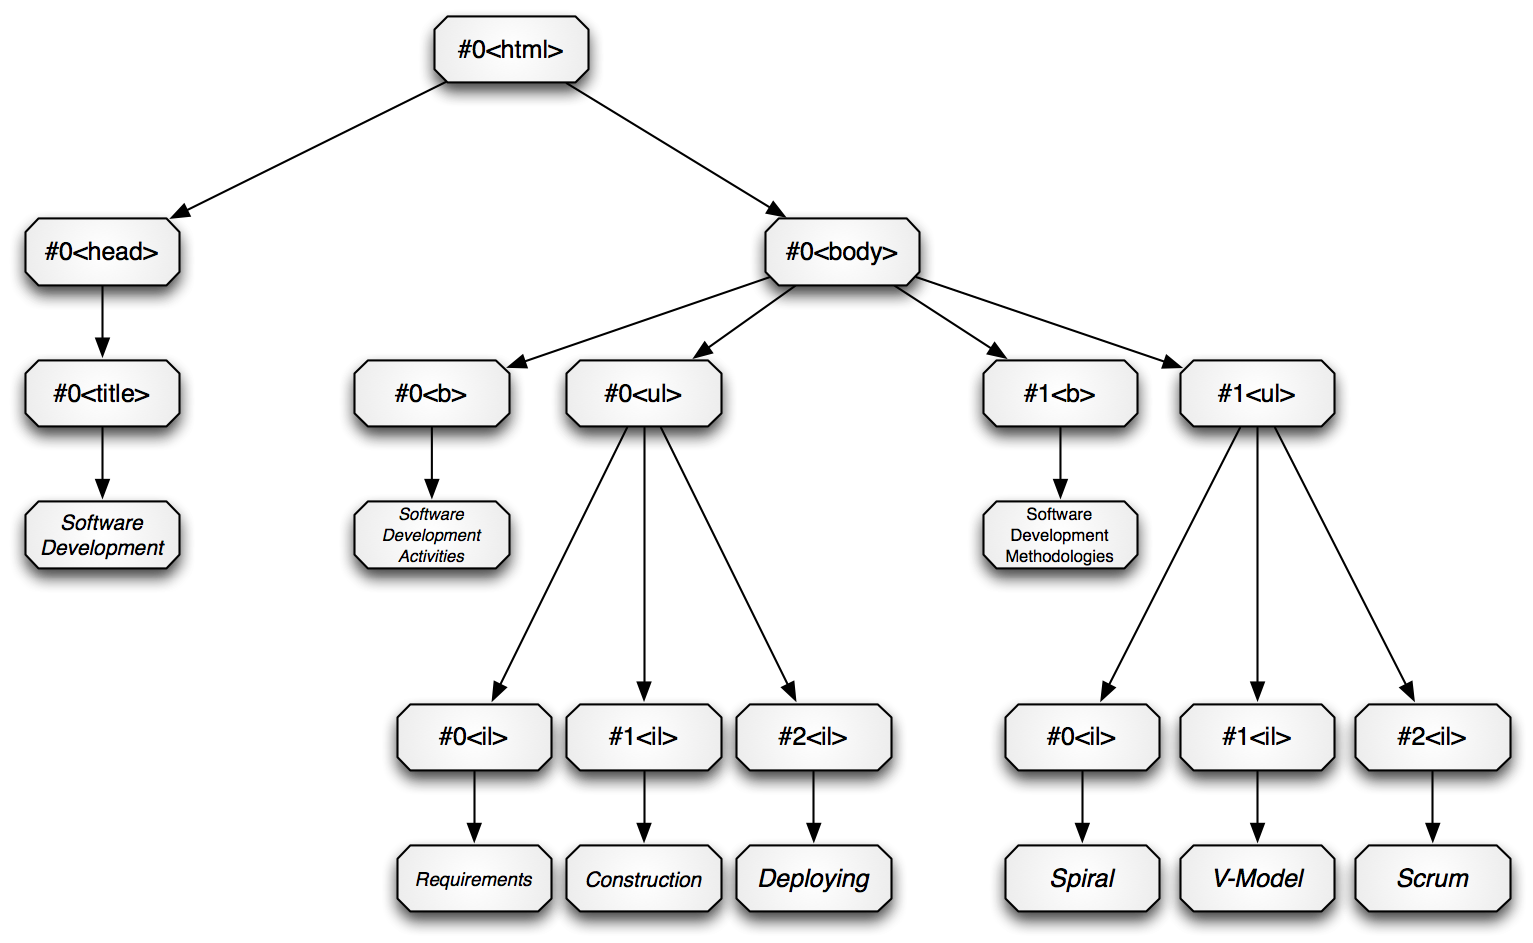
\includegraphics[width=13cm]{images/dom-paramaterized-tree-example.png}
		\caption{Example for parameter DOM tree}
		\label{dom-paramaterized-tree-example}
\end{figure} 

\subsubsection{Effects of Web Evolution Element Matching}

This section compares the script support and parameter DOM path approach in regard to web evolution. Web evolution means any changes that happen to the HTML code we use for element matching. We do not care whether those changes are updates made by user or that happen automatically. Changes are a risk for both approaches so that elements cannot be matched anymore. However, the script support is more robust to changes that appear somewhere not near the elements location. The parameter DOM path might affect on any element anchors.
To show this, we use the HTML example from Figure \ref{dom-html-example}. The element \verb^Construction^ should be matched with the parameter DOM path and a simple script. Then we change the structure of the HTML code and observe the effects on both procedures.

In the previous section we already determined the parameter DOM path for the element \verb^Construction^ which is \verb^\#0<html>,\#0<body>,\#0<ul>,\#1<li>^. This parameter is enough to clearly find the right element. 

As script, we use the text from the content of the element itself and the class type of its immediate parent. The get those information we use the following script:
\begin{lstlisting}
{
    rules:
    [
         {"element_content" : "$(matchedElement).text()"},
         {"element_parent" : "$(matchedElement).parents().first()"}
    ]
}
\end{lstlisting}

Normally we would check on the documents URL to only apply the script to the right environment. In this case, we keep it simple to keep focus on the actual issue. If the script is executed on \verb^Construction^ we retrieve the following results:

\begin{lstlisting}
{
         {"element_content" : "Construction"},
         {"element_parent" : "li"}
}
\end{lstlisting}

The update that happens to the HTML code is a newly inserted element into the \emph{Software Development Activities} list. The new parameter tree is shown in Figure \ref{dom-paramaterized-modified-tree-example}. Even though the matched element \verb^Construction^ is not directly changed, the updated environment results in a new parameter DOM path, which is:
\verb^\#0<html>,\#0<body>,\#0<ul>,\#2<li>^. The changes are slightly different, but still it crashes our matching procedures. \verb^Construction^ cannot be found anymore using the DOM path. 


\begin{figure}\centering
		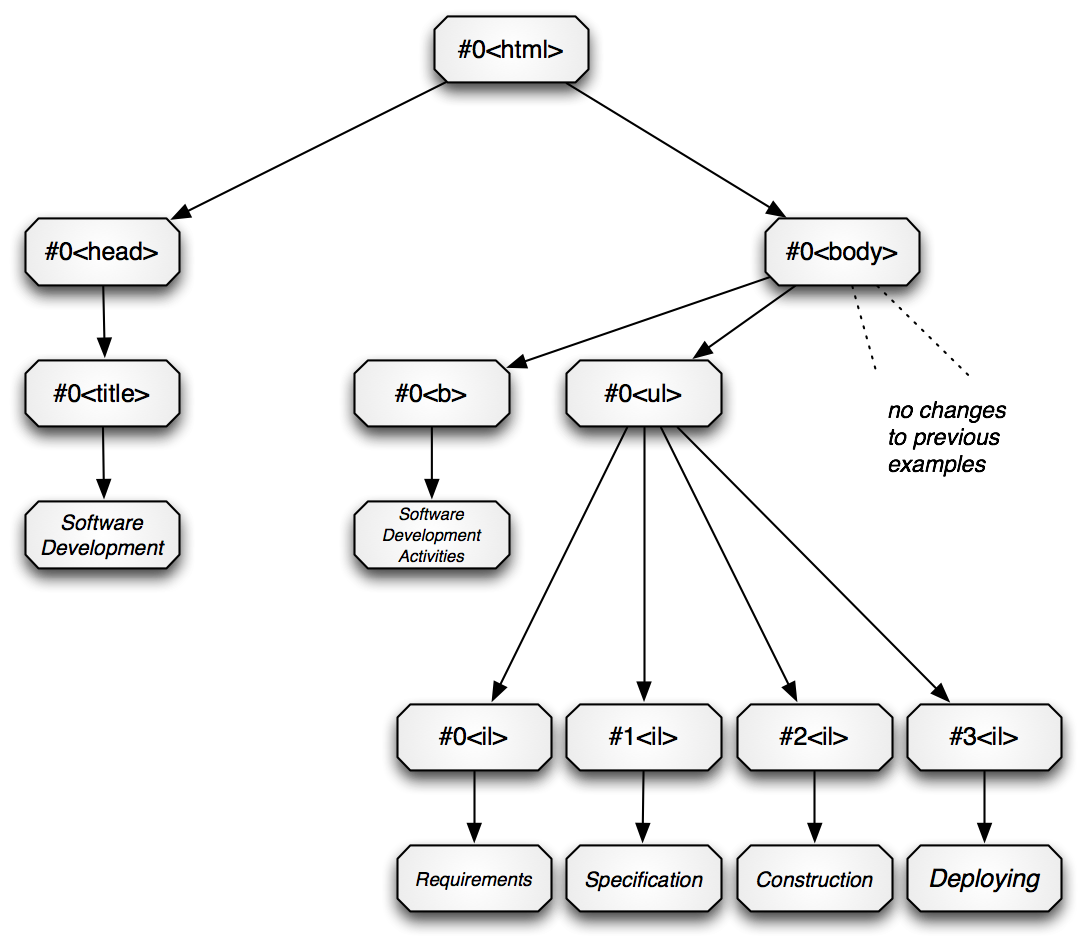
\includegraphics[width=13cm]{images/dom-paramaterized-modified-tree-example.png}
		\caption{Modified parameter DOM tree}
		\label{dom-paramaterized-modified-tree-example}
\end{figure} 

Nevertheless, the script still finds the element correctly since its independent from most of the environment. The results for the script execution we received earlier, does not change. 

\begin{figure}\centering
	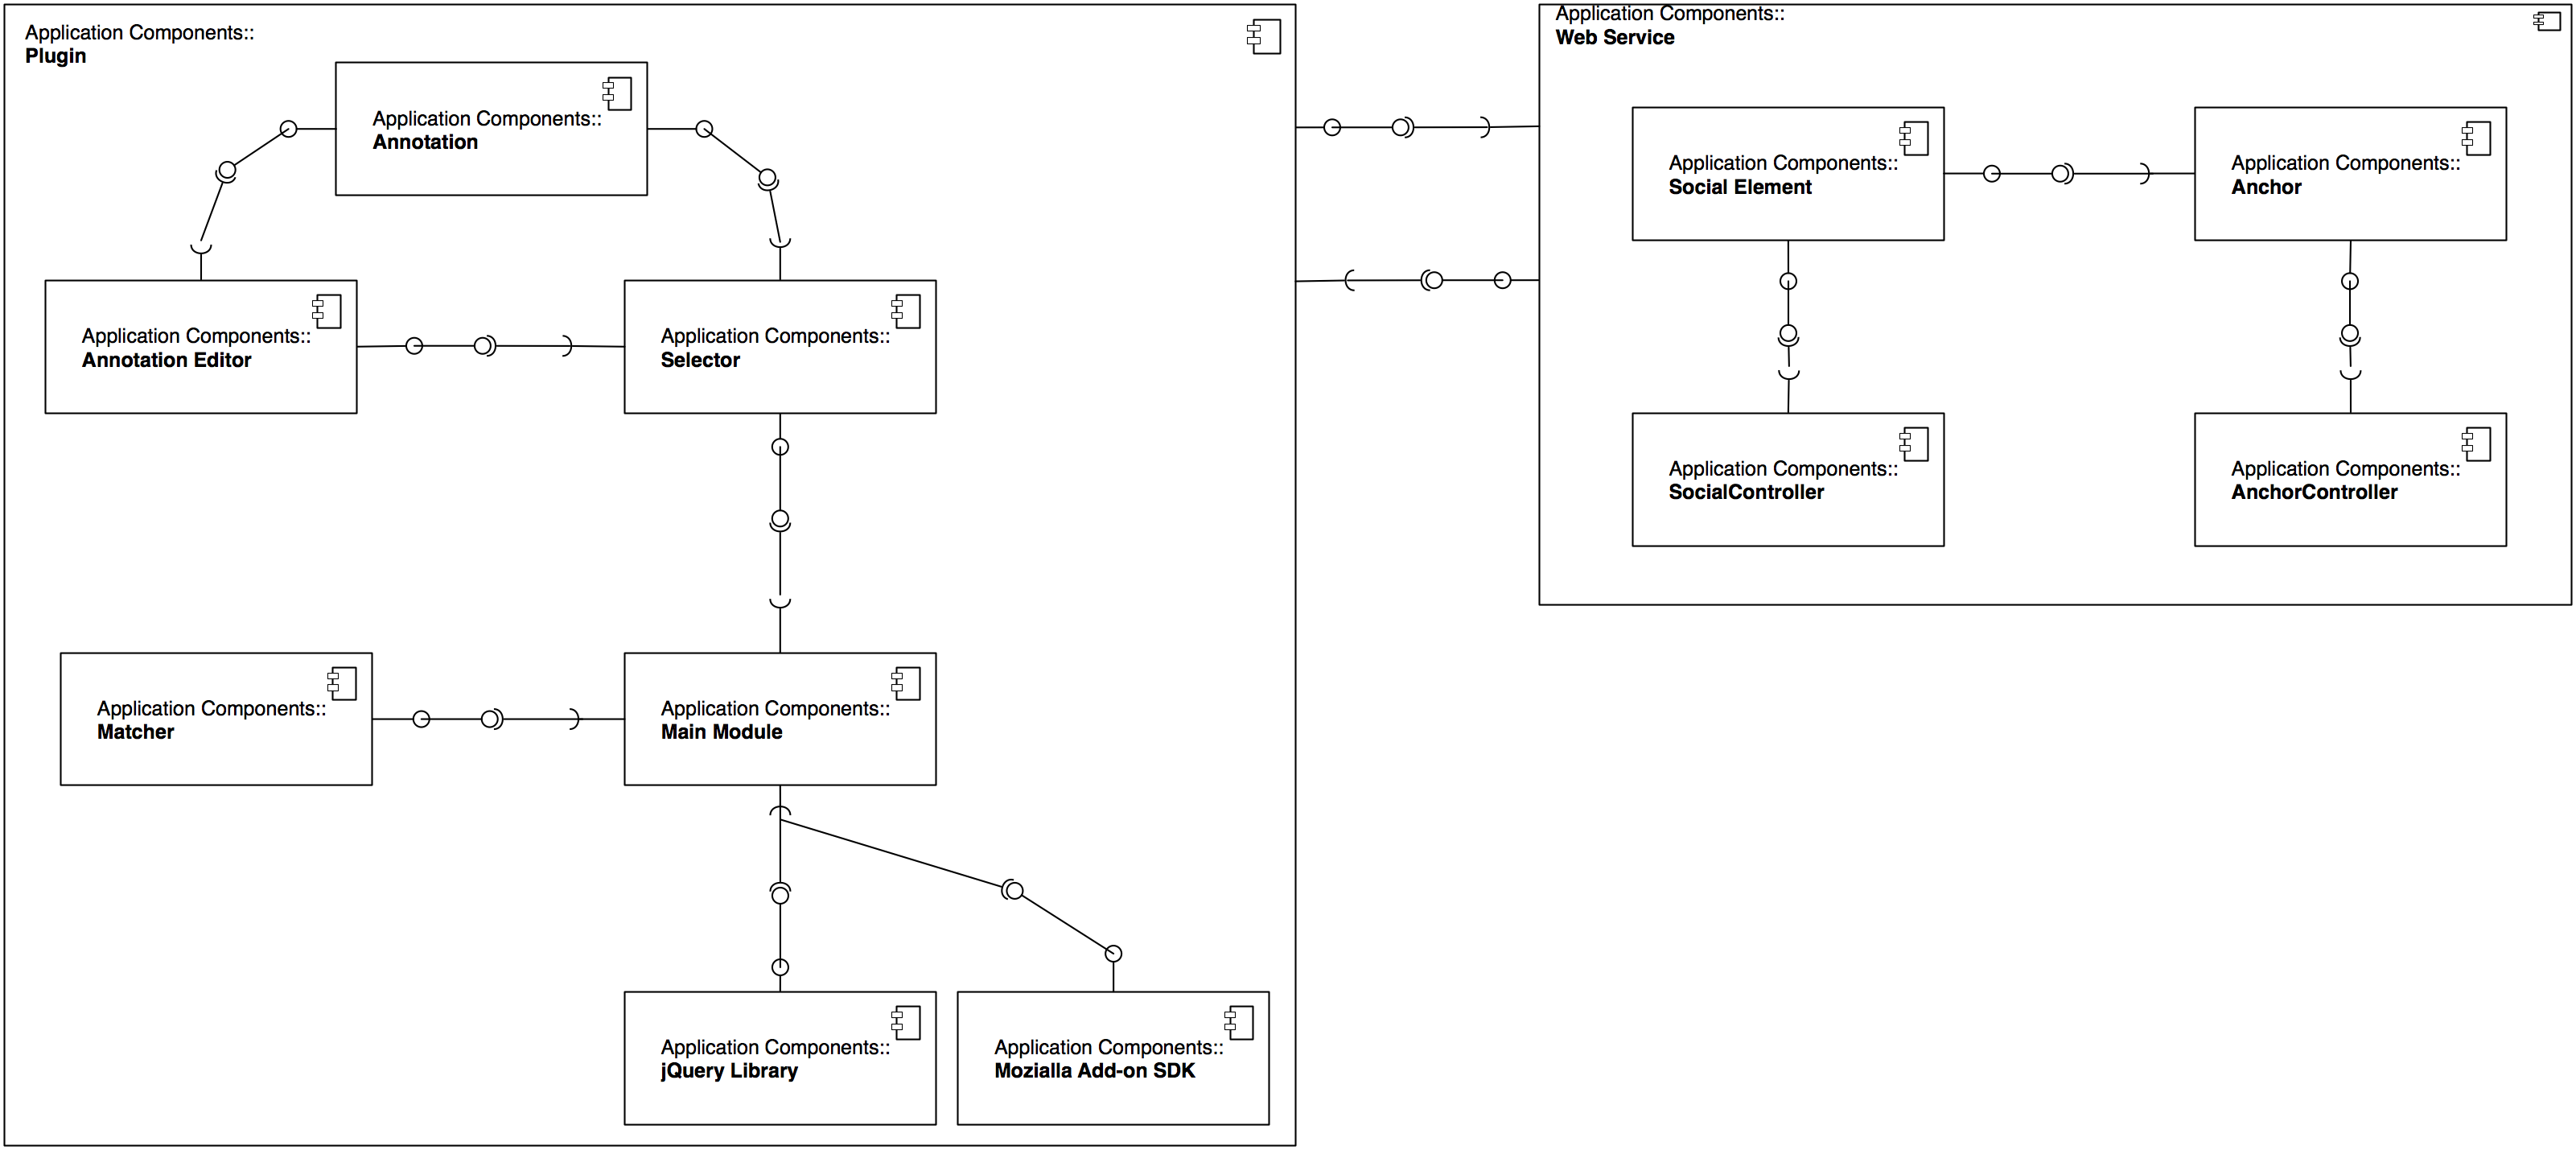
\includegraphics[width=13cm]{images/component-wholesystem-diagram.png}
	\caption{Component diagram for whole system}
	\label{component-wholesystem-diagram}
\end{figure}

Keep in mind that there still are changes that can happen in the HTML code and that would affect scripts. There simply is no guarantee for a reliable anchor without exception.

\newpage
%\subsection{Dependencies accross Modules}\label{module-dependencies}
\newpage

\section{Conclusion}

In the abstract concept level we learned what a Social Weaving system needs to provide and what problems might appear. We defined the requirements and roughly an architecture. Using this knowledge in the second part we described an implementation of a prototype on a more detailed and technical level. This should be seen as a proof of concept that Social Weaving is basically possible. 
\newpage

\bibliographystyle{plain}
\bibliography{references}
\nocite{*}

\end{document}